\documentclass[10pt]{article}
\usepackage{comment}
\usepackage[utf8]{inputenc}
\usepackage[T1]{fontenc}
\usepackage{amsmath,amsfonts,amssymb}
\usepackage{graphicx}
\usepackage{caption}
\usepackage{subcaption}
\usepackage{hyperref}
\usepackage{geometry}
\usepackage{fancyhdr}
\usepackage{float}
\usepackage{cite}
\usepackage{listings}
\usepackage{xcolor}
\usepackage{authblk}
\geometry{margin=0.75in}

\title{\textbf{Anomaly Detection with QML: A Benchmark study using different approaches with Pennylane}}

\author[1]{Jacopo Martellotto}
\affil[1]{\small\texttt{j.martellotto@studenti.unipi.it}}
\date{}

\author[2]{Federico Morano}
\affil[2]{\small\texttt{f.morano1@studenti.unipi.it}}
\date{} 

\pagestyle{fancy}
\fancyhf{}
\rhead{\thepage}
\lhead{Quantum Machine Learning Report}

\begin{document}

\maketitle

\section{Introduction}


\section{About Dataset}



\section{Preprocessing}


\section{Classic Machine Learning}
\subsection{Dummy}
\subsection{Decision Tree}
\subsection{AdaBoost}
\subsection{KNN}
\subsection{MLP}
\subsection{Logistic Regression}
\subsection{Random Forest}
\subsection{SVM}



\section{Quantum Machine Learning}
\subsection{QNN}


\subsection{QFNN}
\begin{figure}[h!]
	\centering
	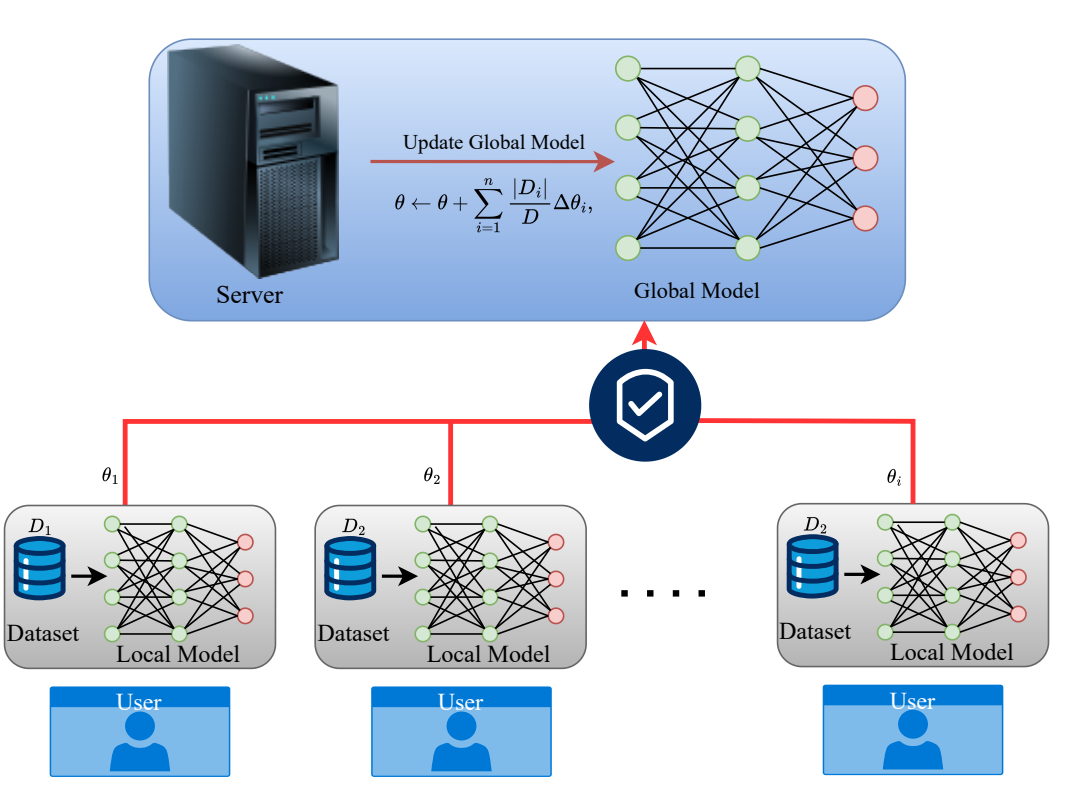
\includegraphics[height = 0.30\textheight]{img/FL_model.png}
	\caption{A schematic overview of the Federated Learning (FL) architecture illustrates several users (clients), each working with their own private dataset to independently train local models. Instead of sharing raw data, clients send their model updates to a central server. The server combines these updates to enhance the global model, which is then redistributed to all clients for the next training round. This iterative process preserves data privacy and security by ensuring that users' raw data remains on their local devices.}
\end{figure}
Federated Learning (FL) has recently gained prominence due to growing concerns about data privacy and the limitations of cloud-based deep learning with large-scale datasets. This learning paradigm involves two main components: a central server and multiple client nodes. The central server maintains the global model and collects the locally trained parameters from client devices. It then aggregates these parameters to update the global model, which is subsequently shared back with all clients. Each client trains the received model using its own local data, which typically represents only a small subset of the overall dataset.
In our proposed framework, the client nodes consist of quantum computers or quantum simulators that train circuit parameters using a hybrid quantum-classical approach. During each training round, a selected group of client nodes carries out local training. Afterward, the updated circuit parameters from all participating clients are sent to the central node, where they are aggregated to refine the global model.
\begin{figure}[h!]
	\centering
	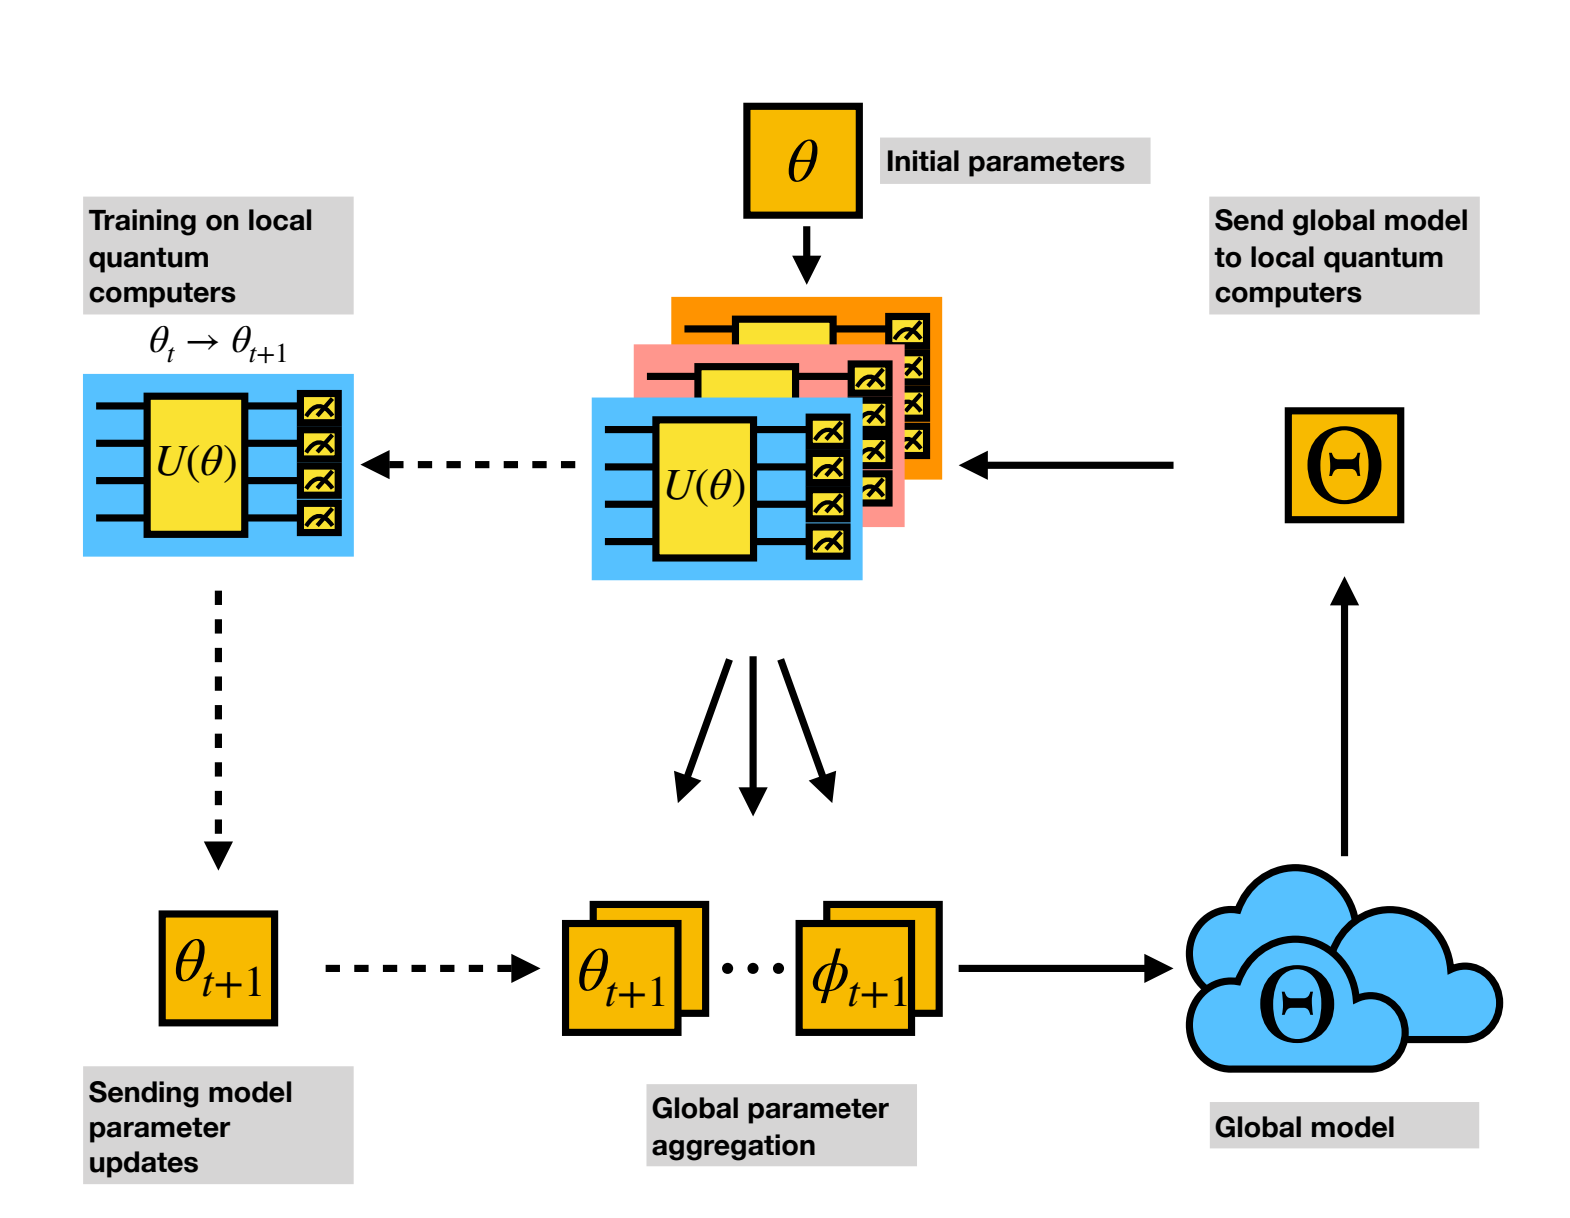
\includegraphics[height = 0.30\textheight]{img/QFL.png}
	\caption{Federated Quantum Learning (QFL)}
\end{figure}
The primary objective of this approach is to develop an advanced fraud detection system across multiple financial institutions using an innovative approach that integrates \textit{Quantum Federated Learning} (QFL) with adaptive federated learning techniques. The proposed solution emphasizes both privacy preservation and improved model performance by combining the computational power of quantum-enhanced models with the collaborative nature of federated learning.\\
This solution enables decentralized model training while ensuring that sensitive financial data remains private and secure. The system incorporates several advanced components, including quantum machine learning, homomorphic encryption, blockchain for model integrity, and a dynamic client-weighting mechanism for adaptive learning.
Let's analyze the architecture and key features of this project in detail:
\begin{itemize}
	\item \textbf{Quantum Federated Learning (QFL)}: Integrates quantum computing techniques within a federated learning framework to enhance model training at client nodes using quantum neural networks (QNNs).
	\item \textbf{Privacy Preservation}: Sensitive data remains on local devices and is never shared directly. Security is ensured using homomorphic encryption, quantum key distribution (QKD), and secret sharing protocols, preventing unauthorized access to model updates.
	\item \textbf{Adaptive Federated Learning}: The contribution of each client to the global model is dynamically adjusted based on local performance. Clients with higher accuracy have a greater influence on the aggregation process, thereby improving overall model robustness.
	\item \textbf{Homomorphic Encryption}: Model updates are encrypted during transmission using homomorphic encryption, which allows arithmetic operations to be performed directly on encrypted data without decryption, ensuring confidentiality throughout the training process.
	\item \textbf{Blockchain Integration}: Blockchain (Ethereum) is used to store hashed versions of the aggregated model weights, ensuring transparency, auditability, and protection against tampering through an immutable and decentralized ledger.
\end{itemize}
The implementation of the project relies on a combination of quantum computing libraries, machine learning frameworks, cryptographic techniques, and blockchain technologies:
\begin{itemize}
	\item \textbf{PennyLane}
	\item \textbf{TensorFlow/Keras}
	\item \textbf{TenSEAL}
	\item \textbf{Shamir's Secret Sharing}
	\item \textbf{Ethereum (via Web3)}: A smart contract is deployed to a local Ethereum test network (simulated using Ganache) to store and verify the integrity of model updates in a tamper-proof, decentralized manner.
	\item \textbf{Quantum Key Distribution (QKD)}: Simulated QKD is used for secure key exchange between clients, allowing encrypted communication channels for transmitting model updates securely across the network.
	\item \textbf{SMOTE (Synthetic Minority Oversampling Technique)}
\end{itemize}


\subsubsection{Adaptive Federated Learning Workflow}
The federated learning process is executed in multiple rounds and consists of the following key stages:
\begin{enumerate}
	\item \textbf{Local Training}: Each client trains a hybrid quantum-classical model locally using their own dataset. The data remains on the client’s device and is never shared externally. The resulting model updates are encrypted using homomorphic encryption.
	\item \textbf{Adaptive Client Selection}: Clients are evaluated based on their local performance on a validation set. Only clients exceeding a predefined accuracy threshold are selected to contribute to the global model, ensuring high-quality updates.
	\item \textbf{Weighted Aggregation}: Selected clients send their encrypted updates, which are then aggregated using a performance-weighted average. This process gives more influence to models that demonstrate higher accuracy, thereby enhancing the overall performance of the global model.
	\item \textbf{Secure Communication and Encryption}: Encrypted model updates are transmitted using keys securely exchanged through simulated QKD. Shamir's Secret Sharing is applied to split model parameters, enhancing data confidentiality.
	\item \textbf{Blockchain Verification}: The aggregated global model weights are hashed using a quantum-resistant function (Qhash) and stored on a blockchain. This ensures the integrity and immutability of the model update history, making the learning process auditable and tamper-proof.
	\item \textbf{Global Model Update}: The decrypted aggregated model is used to update the global model, which is then redistributed to clients for the next round of training.
\end{enumerate}
This architecture successfully achieves a balance between data privacy, system transparency, and high model performance. By enabling multiple financial institutions to collaboratively train a fraud detection model without exposing sensitive data, the proposed system addresses critical security and trust issues in distributed machine learning applications.
Let's analyze step-by-step the implementation of the proposed architecture, focusing on the key components and their interactions.

\subsubsection*{- Initialization of Federated Learning Parameters}
The following variables define the core configuration of the federated learning system and its underlying cryptographic mechanisms:
\begin{itemize}
	\item \texttt{ITERATIONS = 3} sets the number of global training rounds that the federated system will perform. Each iteration involves local training on client devices followed by a secure aggregation step at the central server. At the begining, this variable was set to 5, but the maximum accuracy was reached after 3 iterations, so we decided to reduce the number of iterations to 3.
	\item \texttt{\detokenize{NUM_CLIENTS = 10}} defines the total number of clients (or nodes) participating in the federated learning process. These clients will each contribute to training the global model using their local data.
	\item \texttt{PRIME = 104729} specifies a large prime number used as the modulus in the implementation of Shamir’s Secret Sharing. All polynomial evaluations and modular arithmetic in the secret sharing scheme are performed in the finite field defined by this prime, ensuring both security and mathematical correctness.
	\item \texttt{THRESHOLD = 3} sets the minimum number of shares required to reconstruct the original secret in the $(k, n)$ threshold scheme of Shamir. In this configuration, any group of at least 3 out of the 10 clients is sufficient to recover the secret (e.g., a private decryption key), while fewer than 3 shares reveal no information.
\end{itemize}


\subsubsection*{- Secure Model Handling: Shamir's Secret Sharing, Homomorphic Encryption, and Hashing}
\begin{figure}[H]
	\centering
	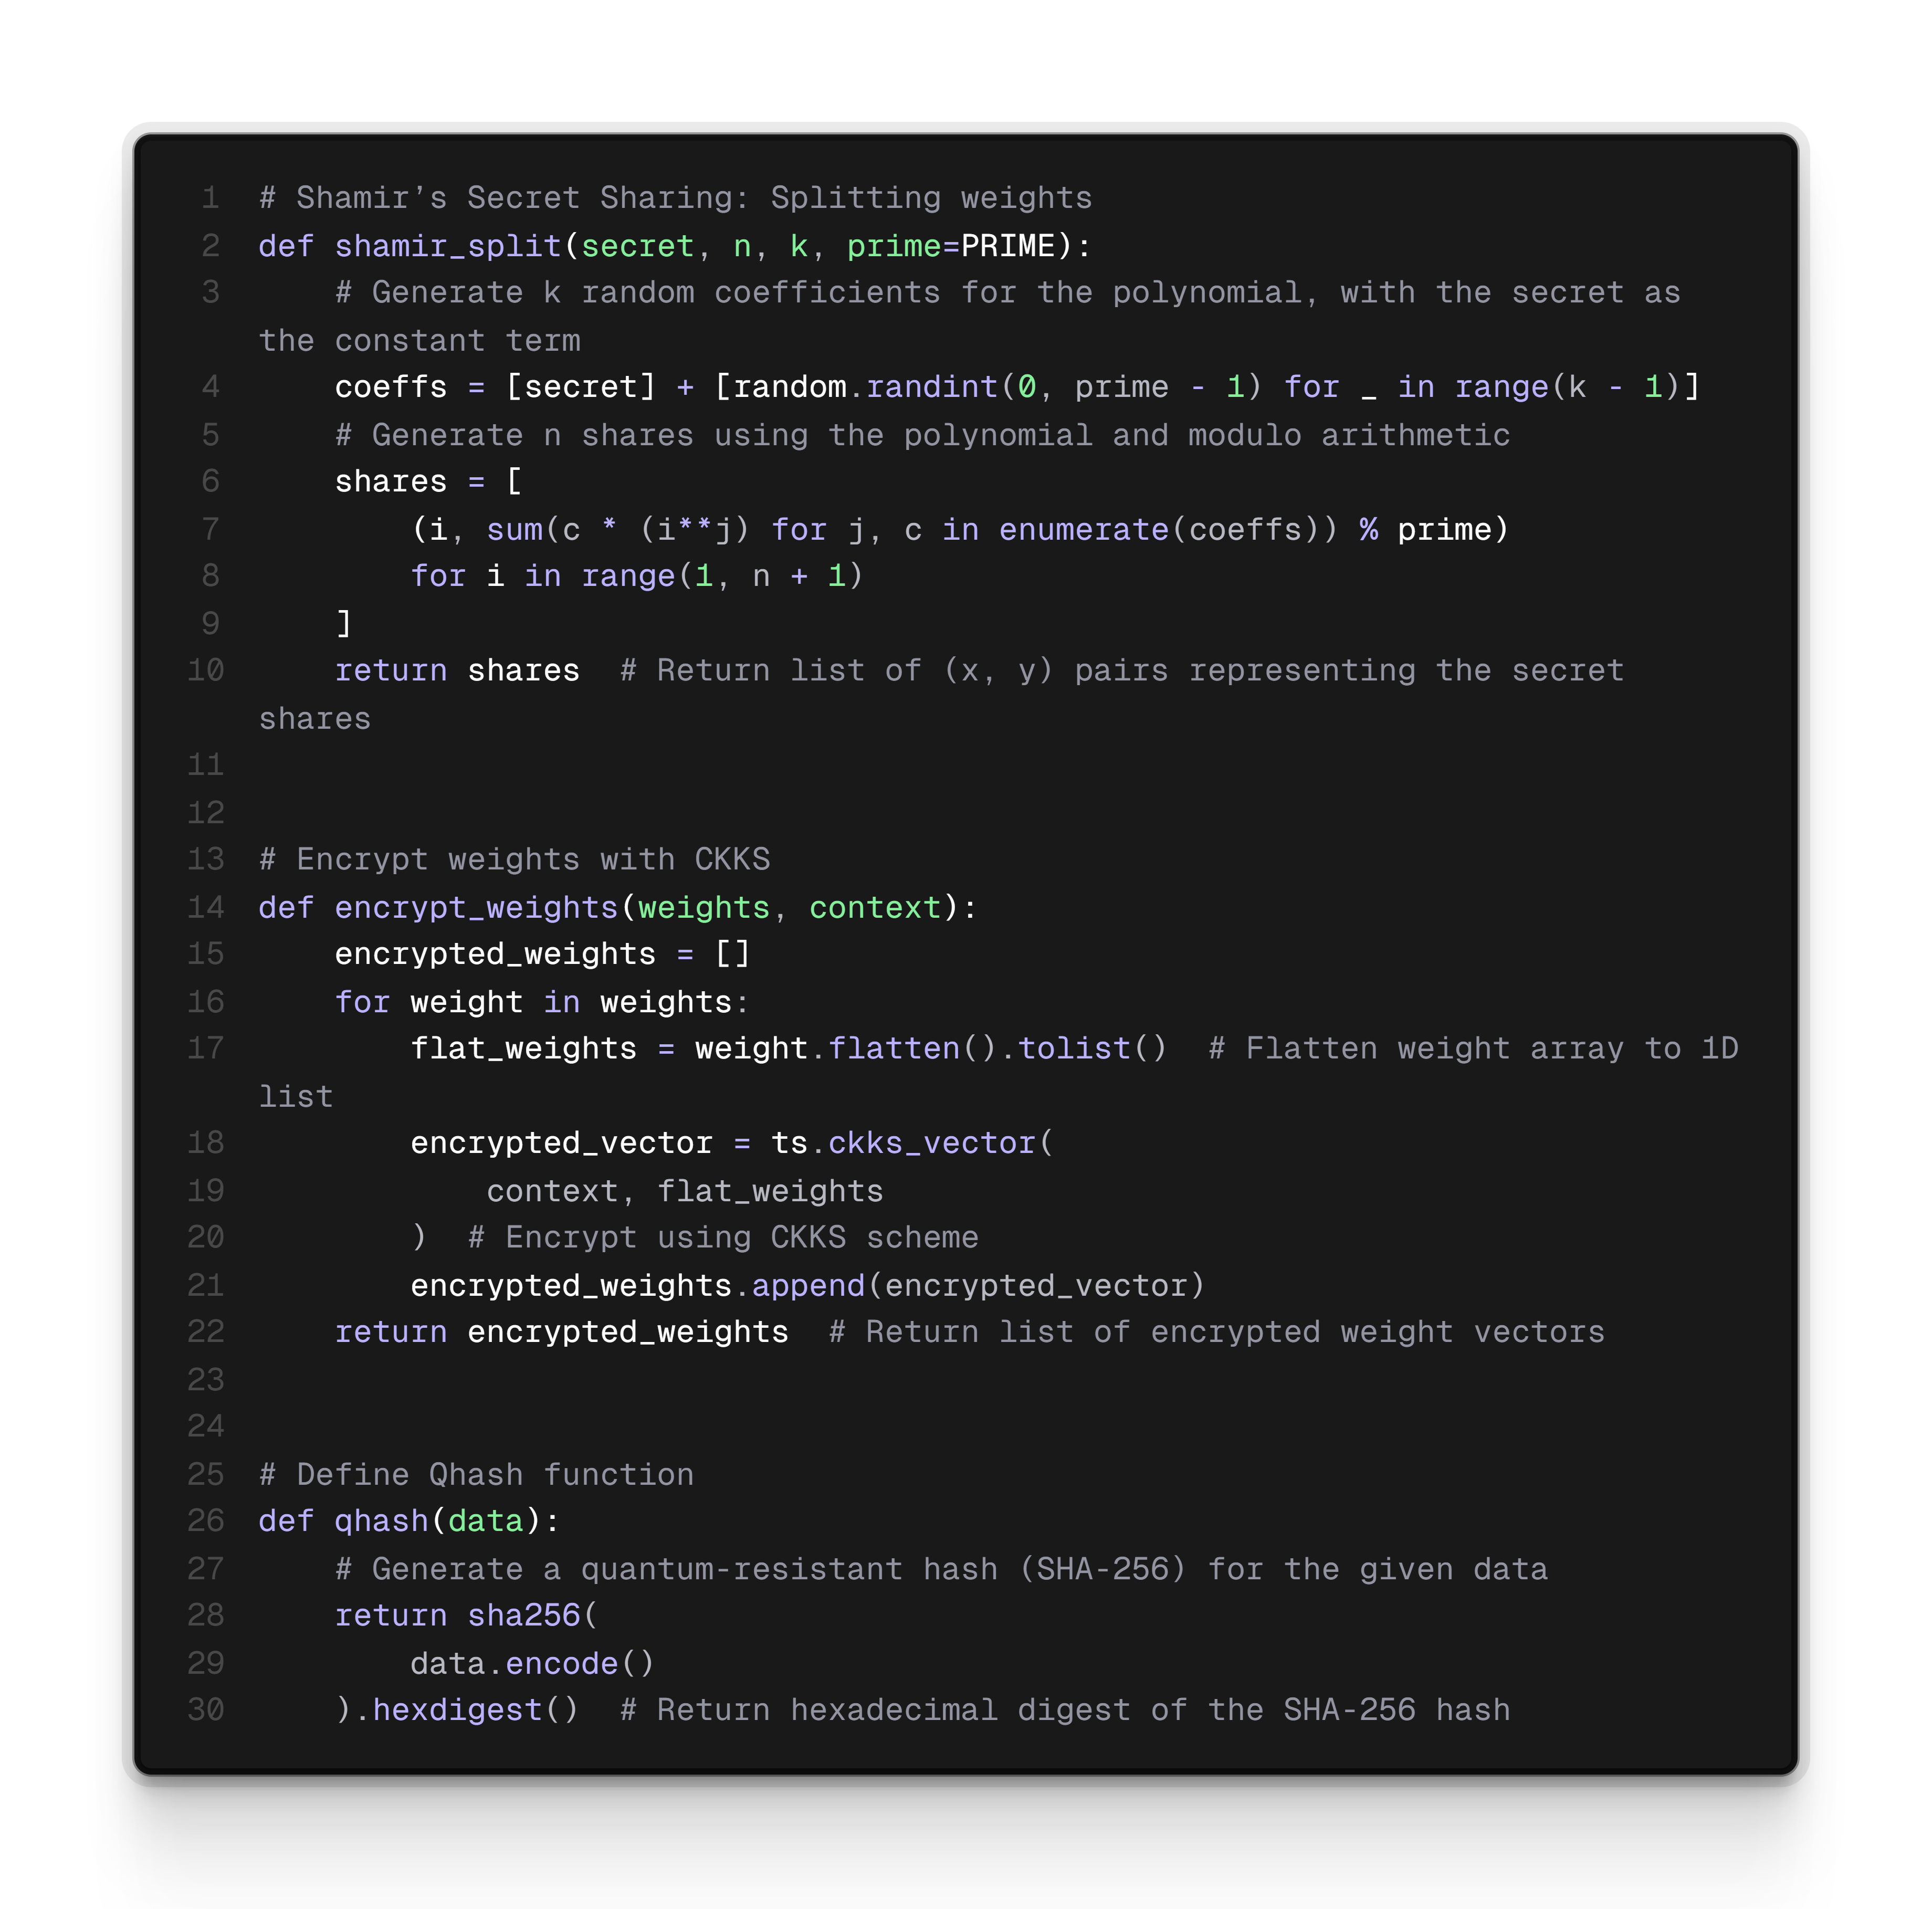
\includegraphics[height = 0.47\textheight]{img/QFL_code/1.png}
\end{figure}
The code segment implements three critical components for securing the parameters and communication of a federated learning system: Shamir’s Secret Sharing, CKKS homomorphic encryption, and a quantum-resistant hash function.\\
The function \texttt{shamir\_split(secret, n, k, prime)} is used to split a sensitive value, such as a model weight or a cryptographic key, into $n$ distinct shares using \textbf{Shamir’s Secret Sharing} scheme. It first generates a random polynomial of degree $k-1$ with the secret as the constant term, and evaluates it at $n$ different $x$-coordinates. Each share corresponds to a unique point $(x, y)$ on this polynomial. The shares can be safely distributed to different clients or nodes. Only when at least $k$ shares are combined can the original secret be reconstructed, ensuring threshold-based access control.\\
The \texttt{encrypt\_weights(weights, context)} function is responsible for encrypting the weights of a machine learning model using the \textbf{CKKS} (Cheon-Kim-Kim-Song) encryption scheme. CKKS supports approximate arithmetic on encrypted floating-point numbers, making it ideal for secure computation in machine learning workflows. Each weight tensor is first flattened and converted to a list, then encrypted using the TenSEAL library’s \texttt{ts.ckks\_vector} method, with the encryption context providing the necessary keys and parameters.\\
Finally, the \texttt{qhash(data)} function generates a \textbf{quantum-resistant cryptographic hash} of the given input string using the SHA-256 algorithm. This function encodes the input to bytes and returns a hexadecimal representation of the 256-bit hash. Although not immune to quantum attacks in the strictest sense, SHA-256 is currently considered sufficiently resistant for practical post-quantum security applications.



\subsubsection*{- Secure Aggregation and Hashing in Federated Quantum Neural Networks}
\begin{figure}[H]
	\centering
	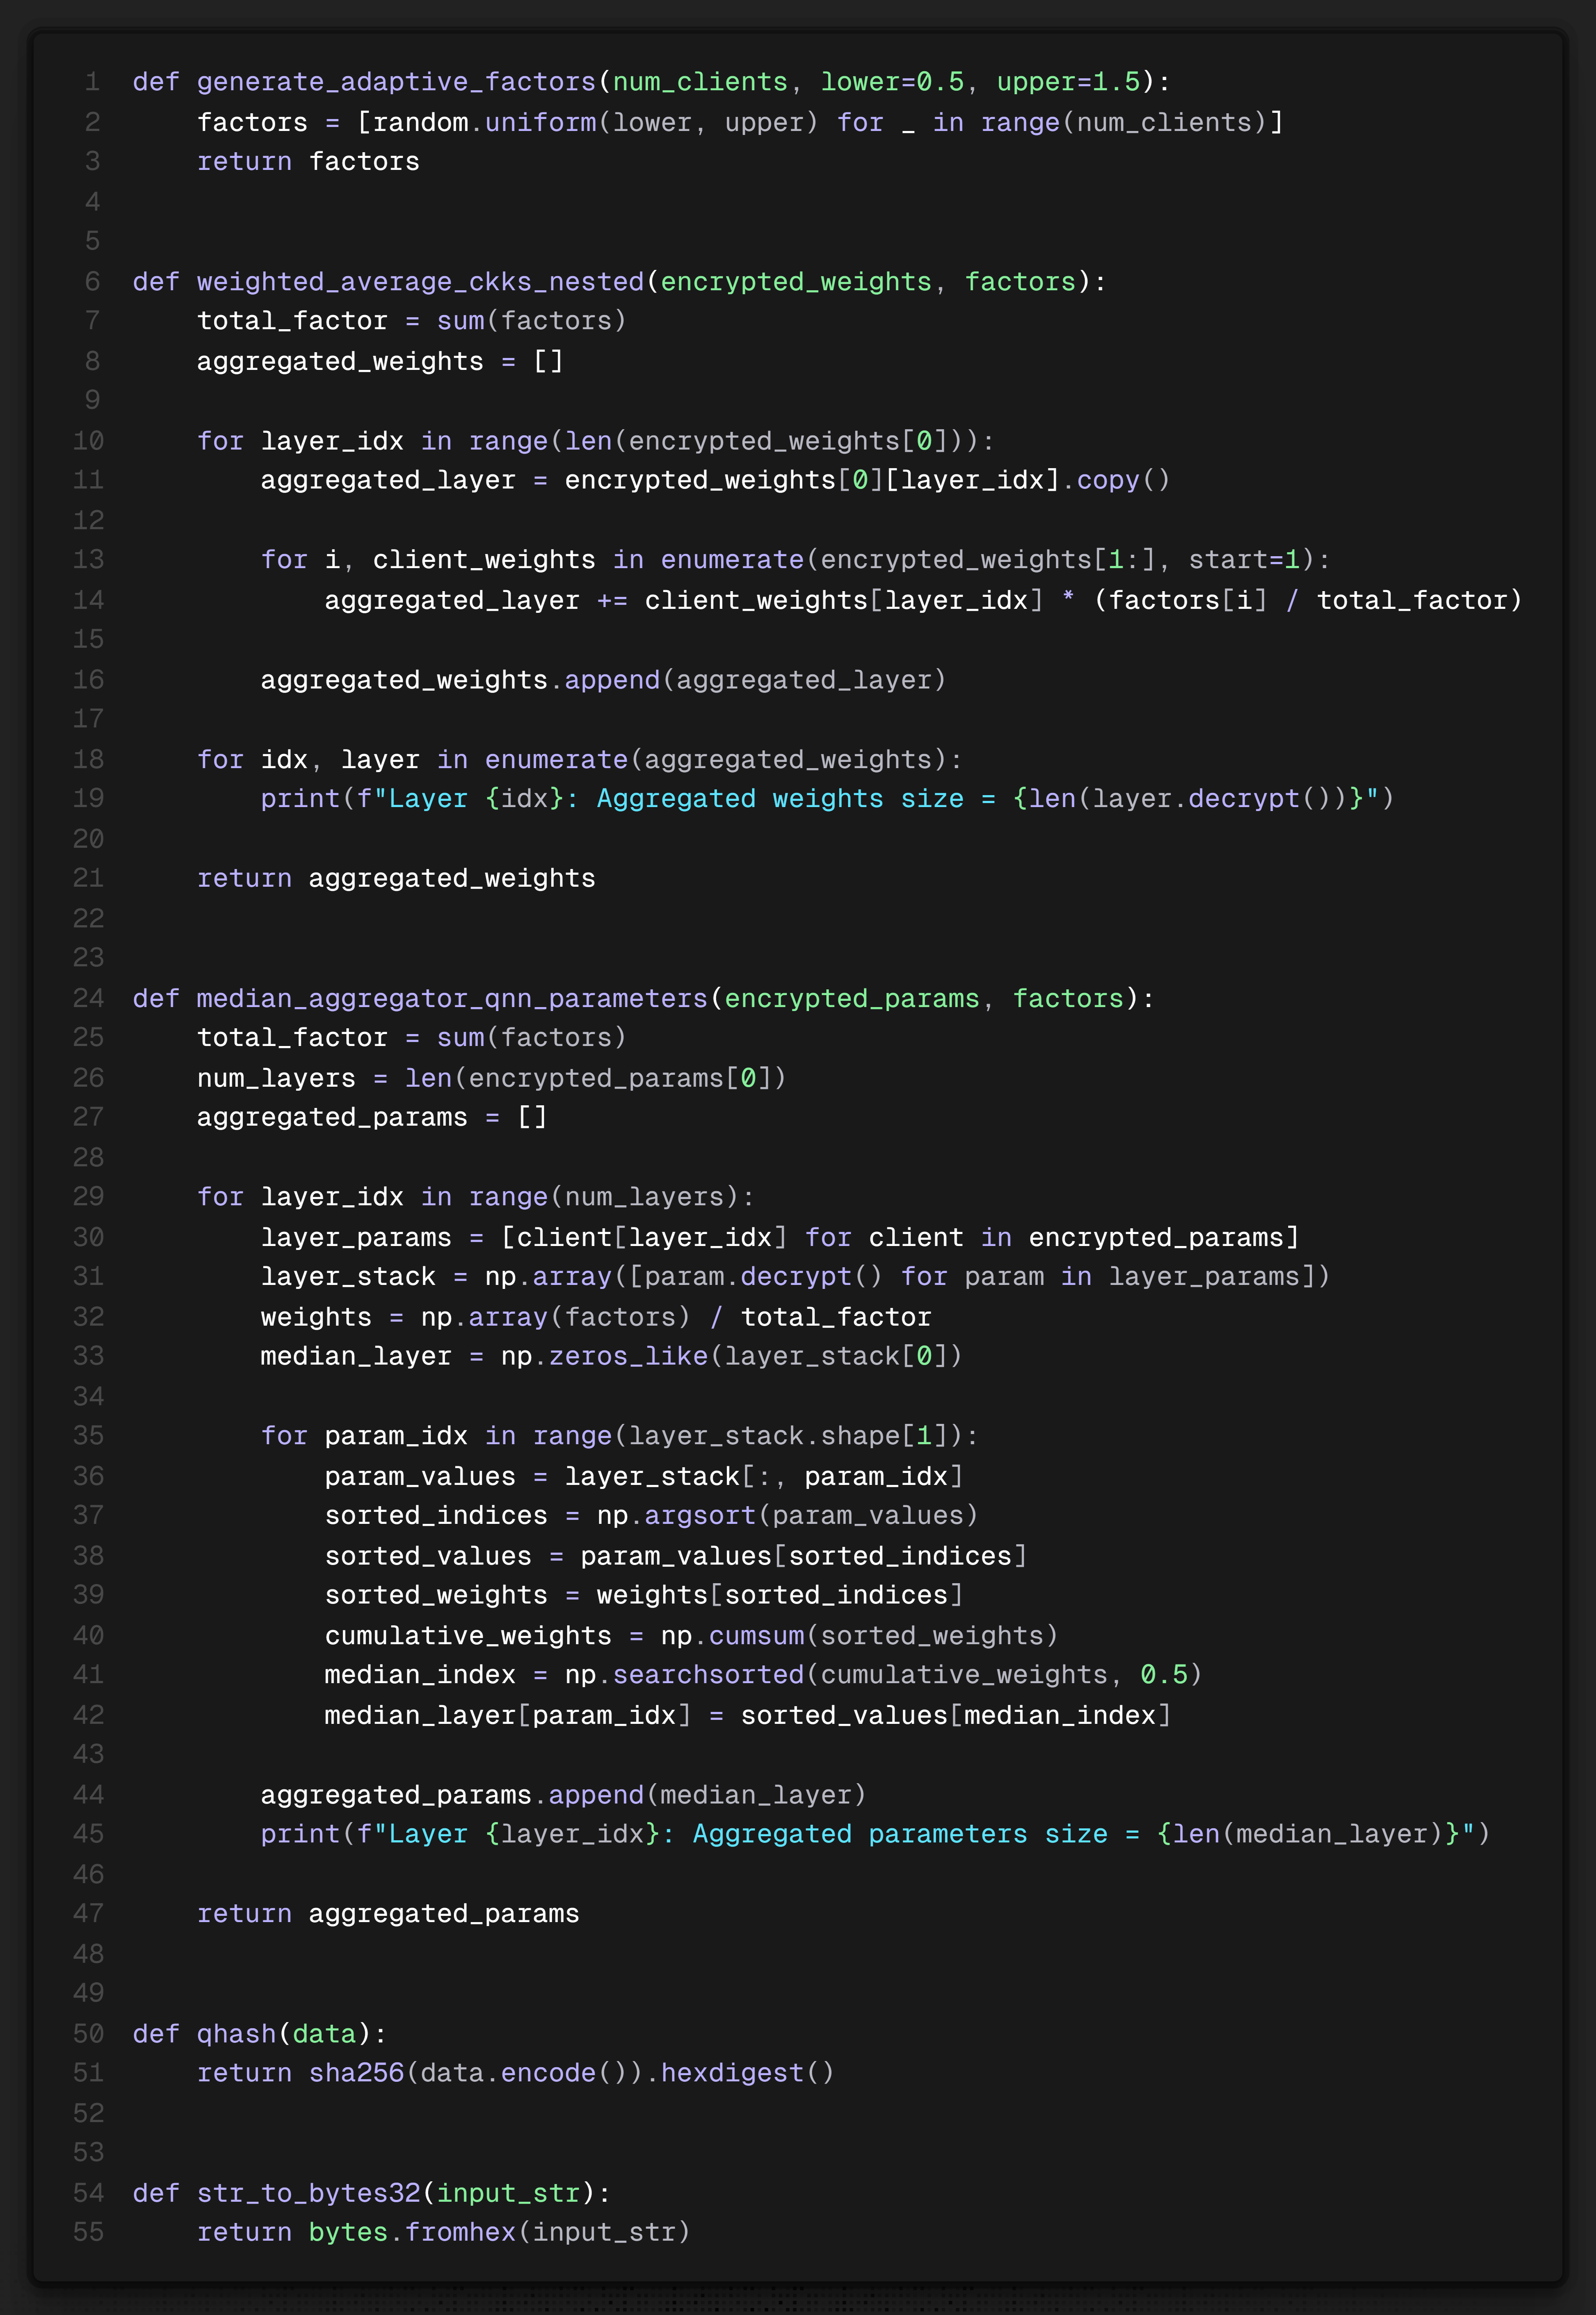
\includegraphics[height = 0.6\textheight]{img/QFL_code/2.png}
\end{figure}
\paragraph{Adaptive Weight Generation}
\texttt{generate\_adaptive\_factors(num\_clients, lower, upper)} generates a list of random floating-point values, one per client, uniformly sampled from a defined range. These values act as \textit{adaptive scaling factors} used to weight each client's contribution during aggregation. Such factors can reflect data quality, sample size, or trustworthiness of each client, and are later normalized when applied to model updates.
\paragraph{Homomorphic Weighted Averaging}
\texttt{weighted\_average\_ckks\_nested(encrypted\_weights, factors)} performs homomorphic aggregation of encrypted model parameters. It assumes that each client's model weights are encrypted using the CKKS scheme and structured as a list of layers. For each layer, it computes a weighted sum across all clients, where each client's weights are scaled by their corresponding adaptive factor. Since the operations are performed directly on encrypted data, the aggregation process ensures strong privacy guarantees. Additionally, the code includes a diagnostic step that decrypts each aggregated layer to log its dimensionality.
\paragraph{Robust Median Aggregation}
\texttt{median\_aggregator\_qnn\_parameters(encrypted\_params, factors)} implements a robust alternative to averaging by computing a weighted median for each parameter across clients. After decrypting each client’s encrypted parameters, the function processes each position (i.e., parameter index) independently: it sorts the values and their associated normalized weights, computes cumulative weights, and selects the parameter value corresponding to the smallest index whose cumulative weight exceeds $0.5$.
\paragraph{Quantum-Resistant Hashing}
\texttt{qhash(data)} computes a cryptographically secure hash of an input string using the SHA-256 algorithm.


\subsection*{- Model Serialization, AES Encryption, and Simulated QKD}
\begin{figure}[H]
	\centering
	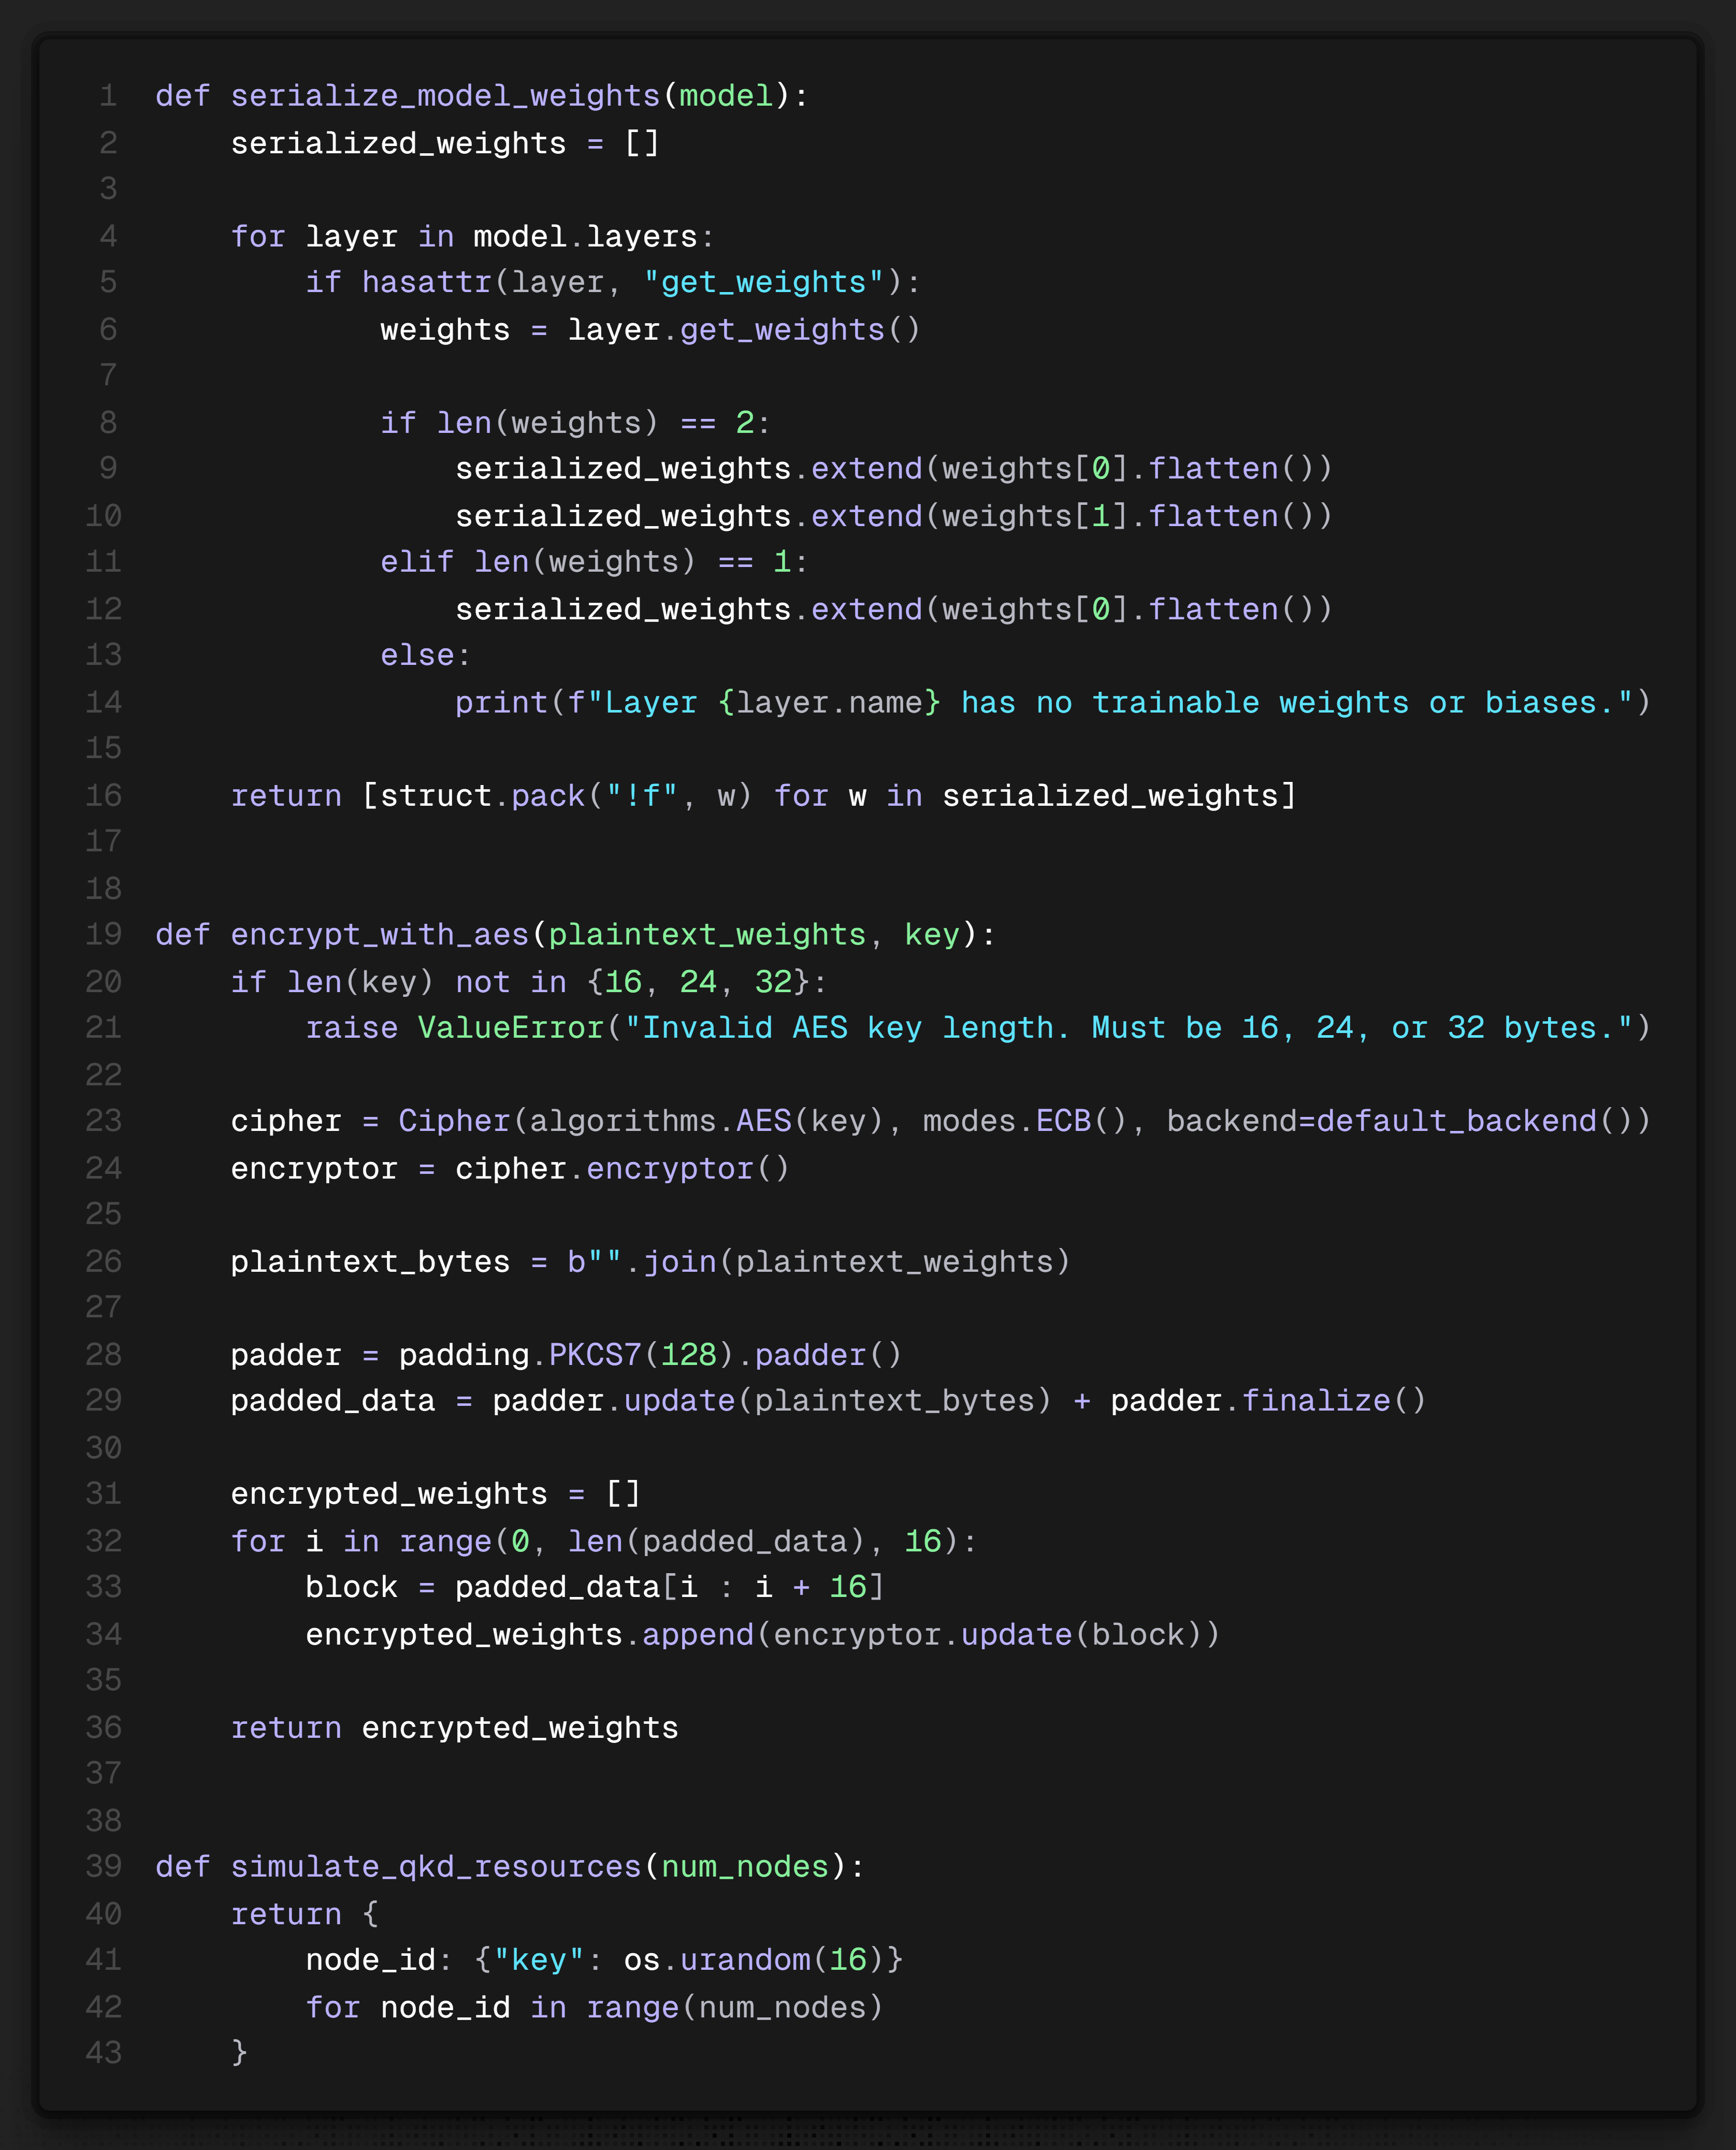
\includegraphics[height = 0.6\textheight]{img/QFL_code/3.png}
\end{figure}
This section introduces a secure pipeline for serializing and encrypting the parameters of a neural network model, along with a simulated key distribution mechanism inspired by Quantum Key Distribution (QKD).
\paragraph{Model Serialization}
\texttt{serialize\_model\_weights(model)} is designed to extract and serialize all trainable parameters (weights and biases) from a Keras-based deep learning model. For each layer in the model, the function checks whether the layer contains trainable parameters via the \texttt{get\_weights()} method. If present, weights and biases are flattened into one-dimensional arrays and added to a list (\texttt{serialized\_weights}). Each floating-point number is then converted into a 4-byte binary representation using the \texttt{struct.pack("!f", w)} instruction, which enforces big-endian byte order. This binary format is compact and compatible with block-based encryption algorithms, such as AES.
\paragraph{AES-Based Encryption}
\texttt{encrypt\_with\_aes(plaintext\_weights, key)} takes the serialized weights (output from the previous function) and encrypts them using AES. The encryption is performed in Electronic Code Book (ECB) mode. Before encryption, the plaintext data is padded using the PKCS7 scheme to align it with AES’s block size (16 bytes). The data is then divided into 16-byte blocks and encrypted individually using the AES cipher. The result is a list of encrypted blocks, each representing a segment of the serialized model parameters.
\paragraph{Simulated QKD for Key Assignment}
\texttt{simulate\_qkd\_resources(num\_nodes)} simulates a Quantum Key Distribution (QKD) system by generating a unique AES key for each client or node in a distributed learning network. The function approximates the output of a QKD protocol by using \texttt{os.urandom} to generate secure, random 128-bit keys. The function returns a dictionary mapping each node identifier to its respective symmetric key.


\subsubsection*{- AES Decryption and Model Weight Deserialization}
\begin{figure}[H]
	\centering
	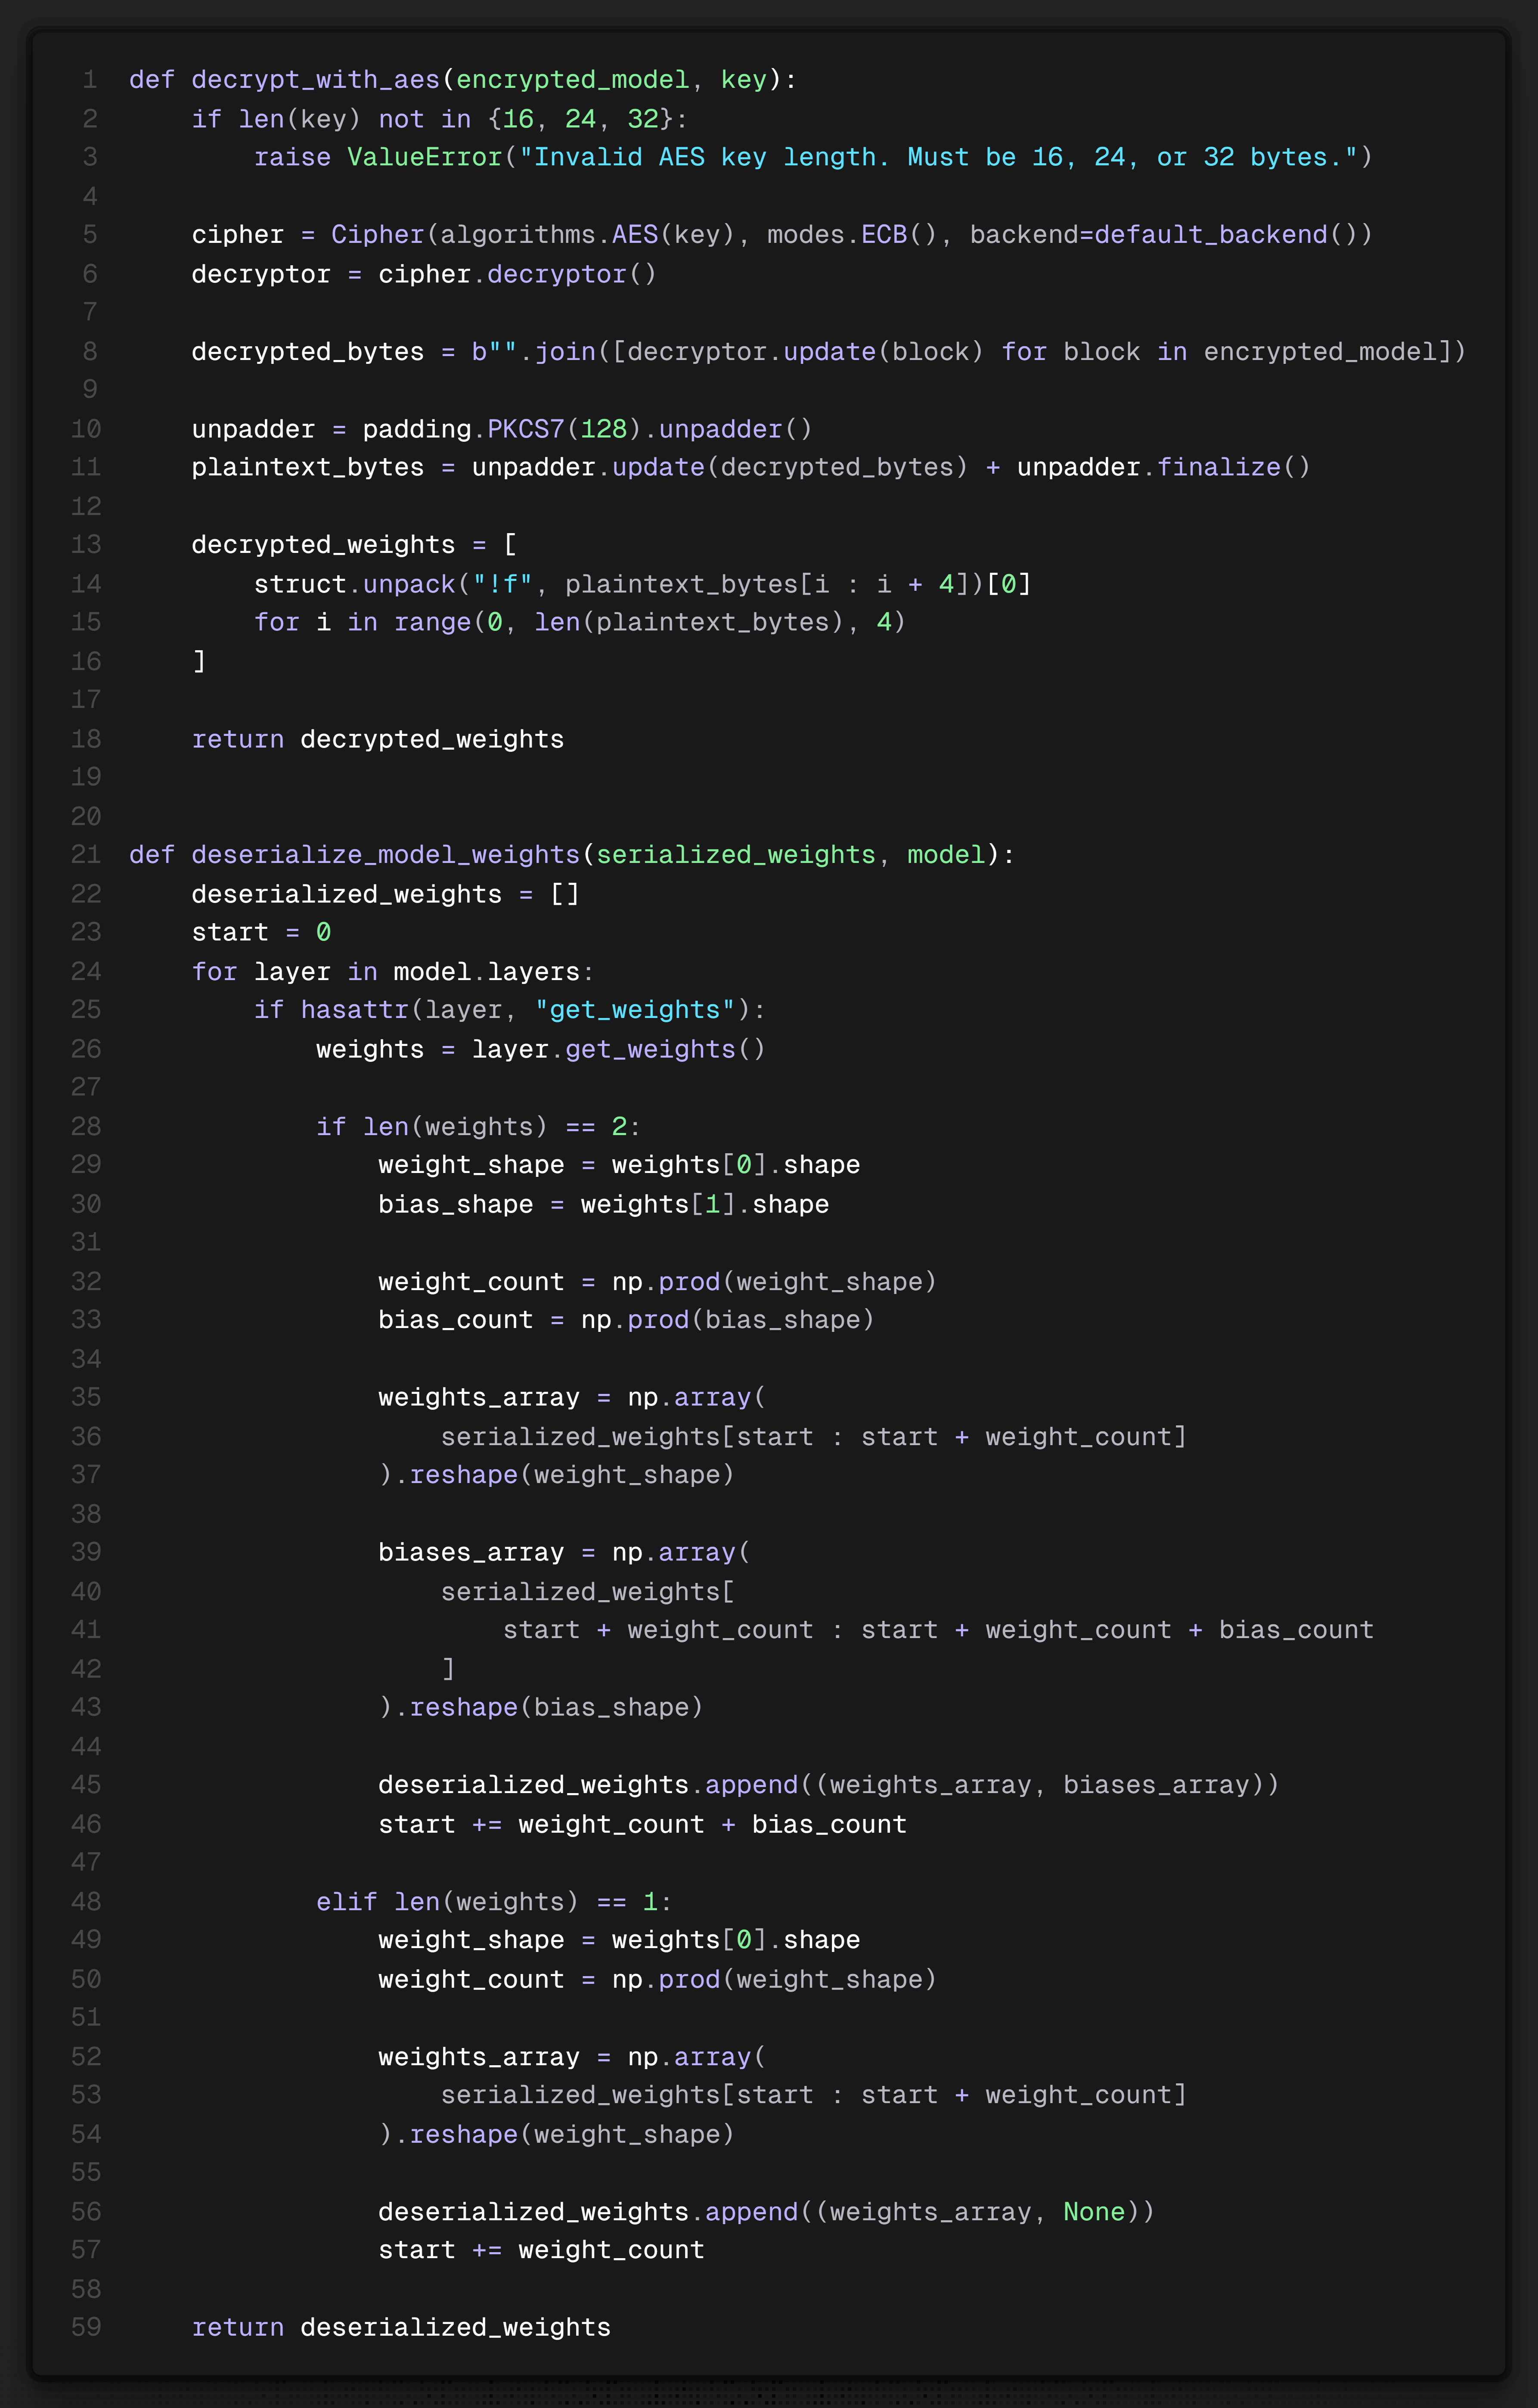
\includegraphics[height = 0.5\textheight]{img/QFL_code/4.png}
\end{figure}
To complete the secure model transmission and reconstruction pipeline, the following functions are used to reverse the encryption and flattening processes previously applied to a neural network's parameters. Specifically, they decrypt AES-encrypted model weights and reshape the flat float list back into tensors compatible with a Keras model's architecture.
\paragraph{AES Decryption of Model Weights}
\texttt{decrypt\_with\_aes(encrypted\_model, key)} is responsible for decrypting a list of AES-encrypted 16-byte blocks. It uses the same symmetric key originally used for encryption and operates in ECB mode. The decryption process begins by concatenating the output of each decrypted block into a single byte string. Since padding was applied during encryption using the PKCS7 scheme, it is removed here to recover the original plaintext size. The raw byte stream is then parsed into 4-byte segments and converted back into 32-bit floating-point values using the \texttt{struct.unpack("!f", ...)} method. The result is a flat list of float values representing the model's parameters.
\paragraph{Weight Deserialization and Model Reconstruction}
\texttt{deserialize\_model\_weights(serialized\_weights, model)} reconstructs the original model weight tensors from a flat list of floating-point values. It assumes that the order and count of weights and biases were preserved during serialization. For each trainable layer in the Keras model, it retrieves the expected shapes of the weights and biases using \texttt{layer.get\_weights()}. It then extracts the appropriate number of elements from the flat list and reshapes them into tensors using NumPy. These are appended as tuples: either \texttt{(weights, biases)} if both exist, or \texttt{(weights, None)} if the layer has no bias terms. A running pointer ensures that the deserialization proceeds sequentially without loss or duplication of data.



\subsubsection*{- Updating Client Models with Global Weights}
\begin{figure}[H]
	\centering
	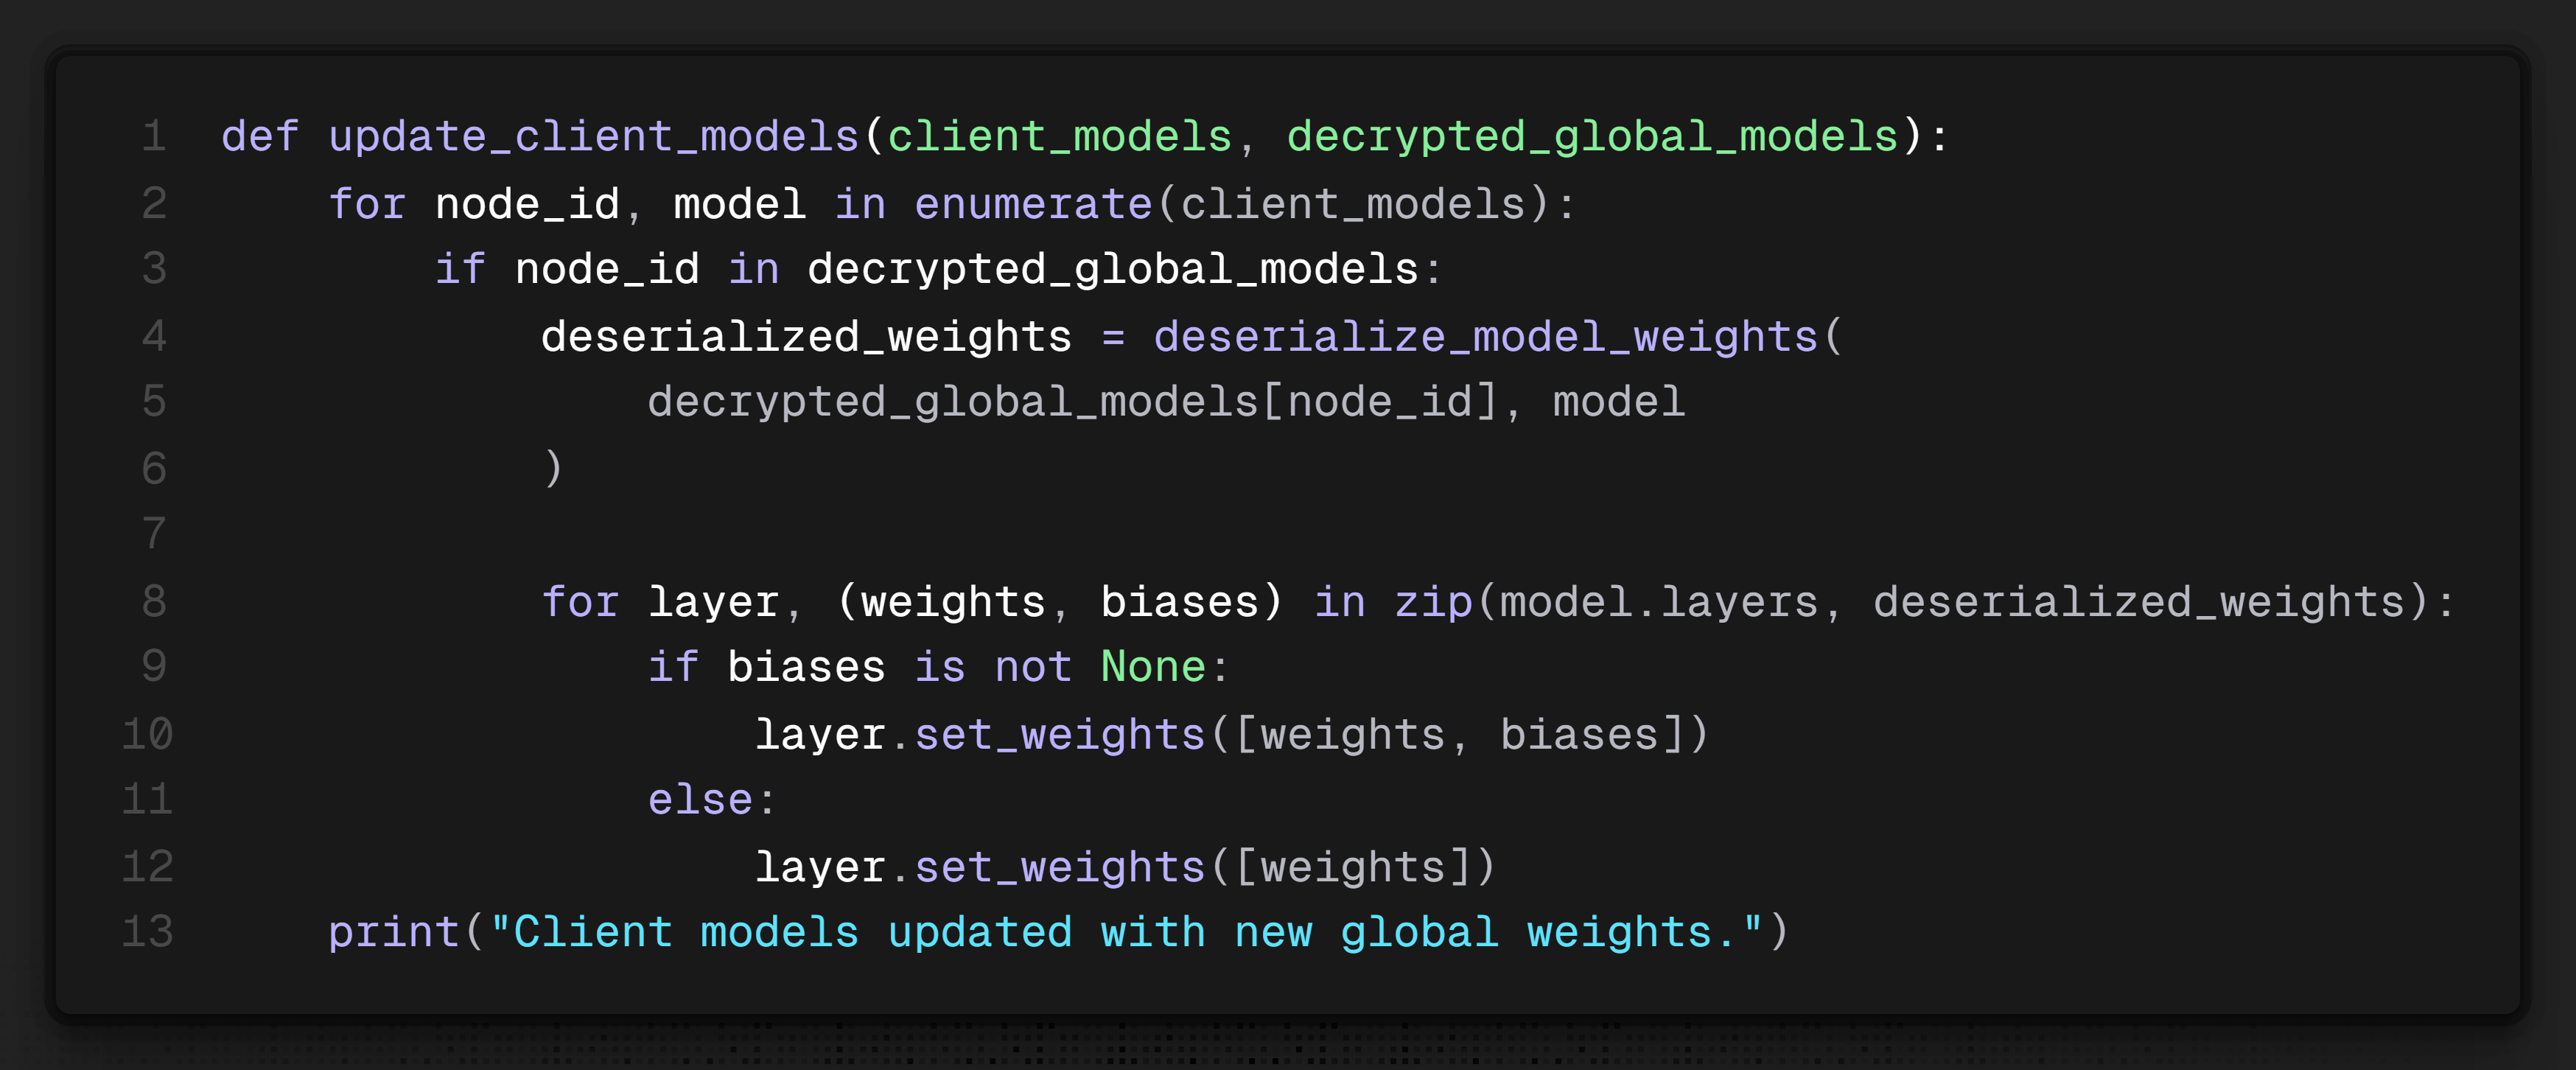
\includegraphics[height = 0.2\textheight]{img/QFL_code/5.png}
\end{figure}
Once the global model weights have been securely aggregated, encrypted, transmitted, and subsequently decrypted by individual clients, the final step is to apply these weights to each client's local model.\\
\texttt{update\_client\_models(client\_models, decrypted\_global\_models)} performs this update process by assigning the appropriate version of the decrypted global model to each client.
Each entry in the \texttt{client\_models} list represents a separate Keras model instance maintained by a client node. The dictionary \texttt{decrypted\_global\_models} maps node IDs to their corresponding sets of decrypted and flattened model weights.


\subsubsection*{- Quantum Layer Structure}
The structure used here is the same as that employed in the QNN. In particular, we use the custom 'long' layer previously described. To avoid redundancy, we refer the reader to the preceding section for a detailed explanation of the quantum layer structure and its implementation.


\subsubsection*{- Local Quantum Model}
\begin{figure}[H]
	\centering
	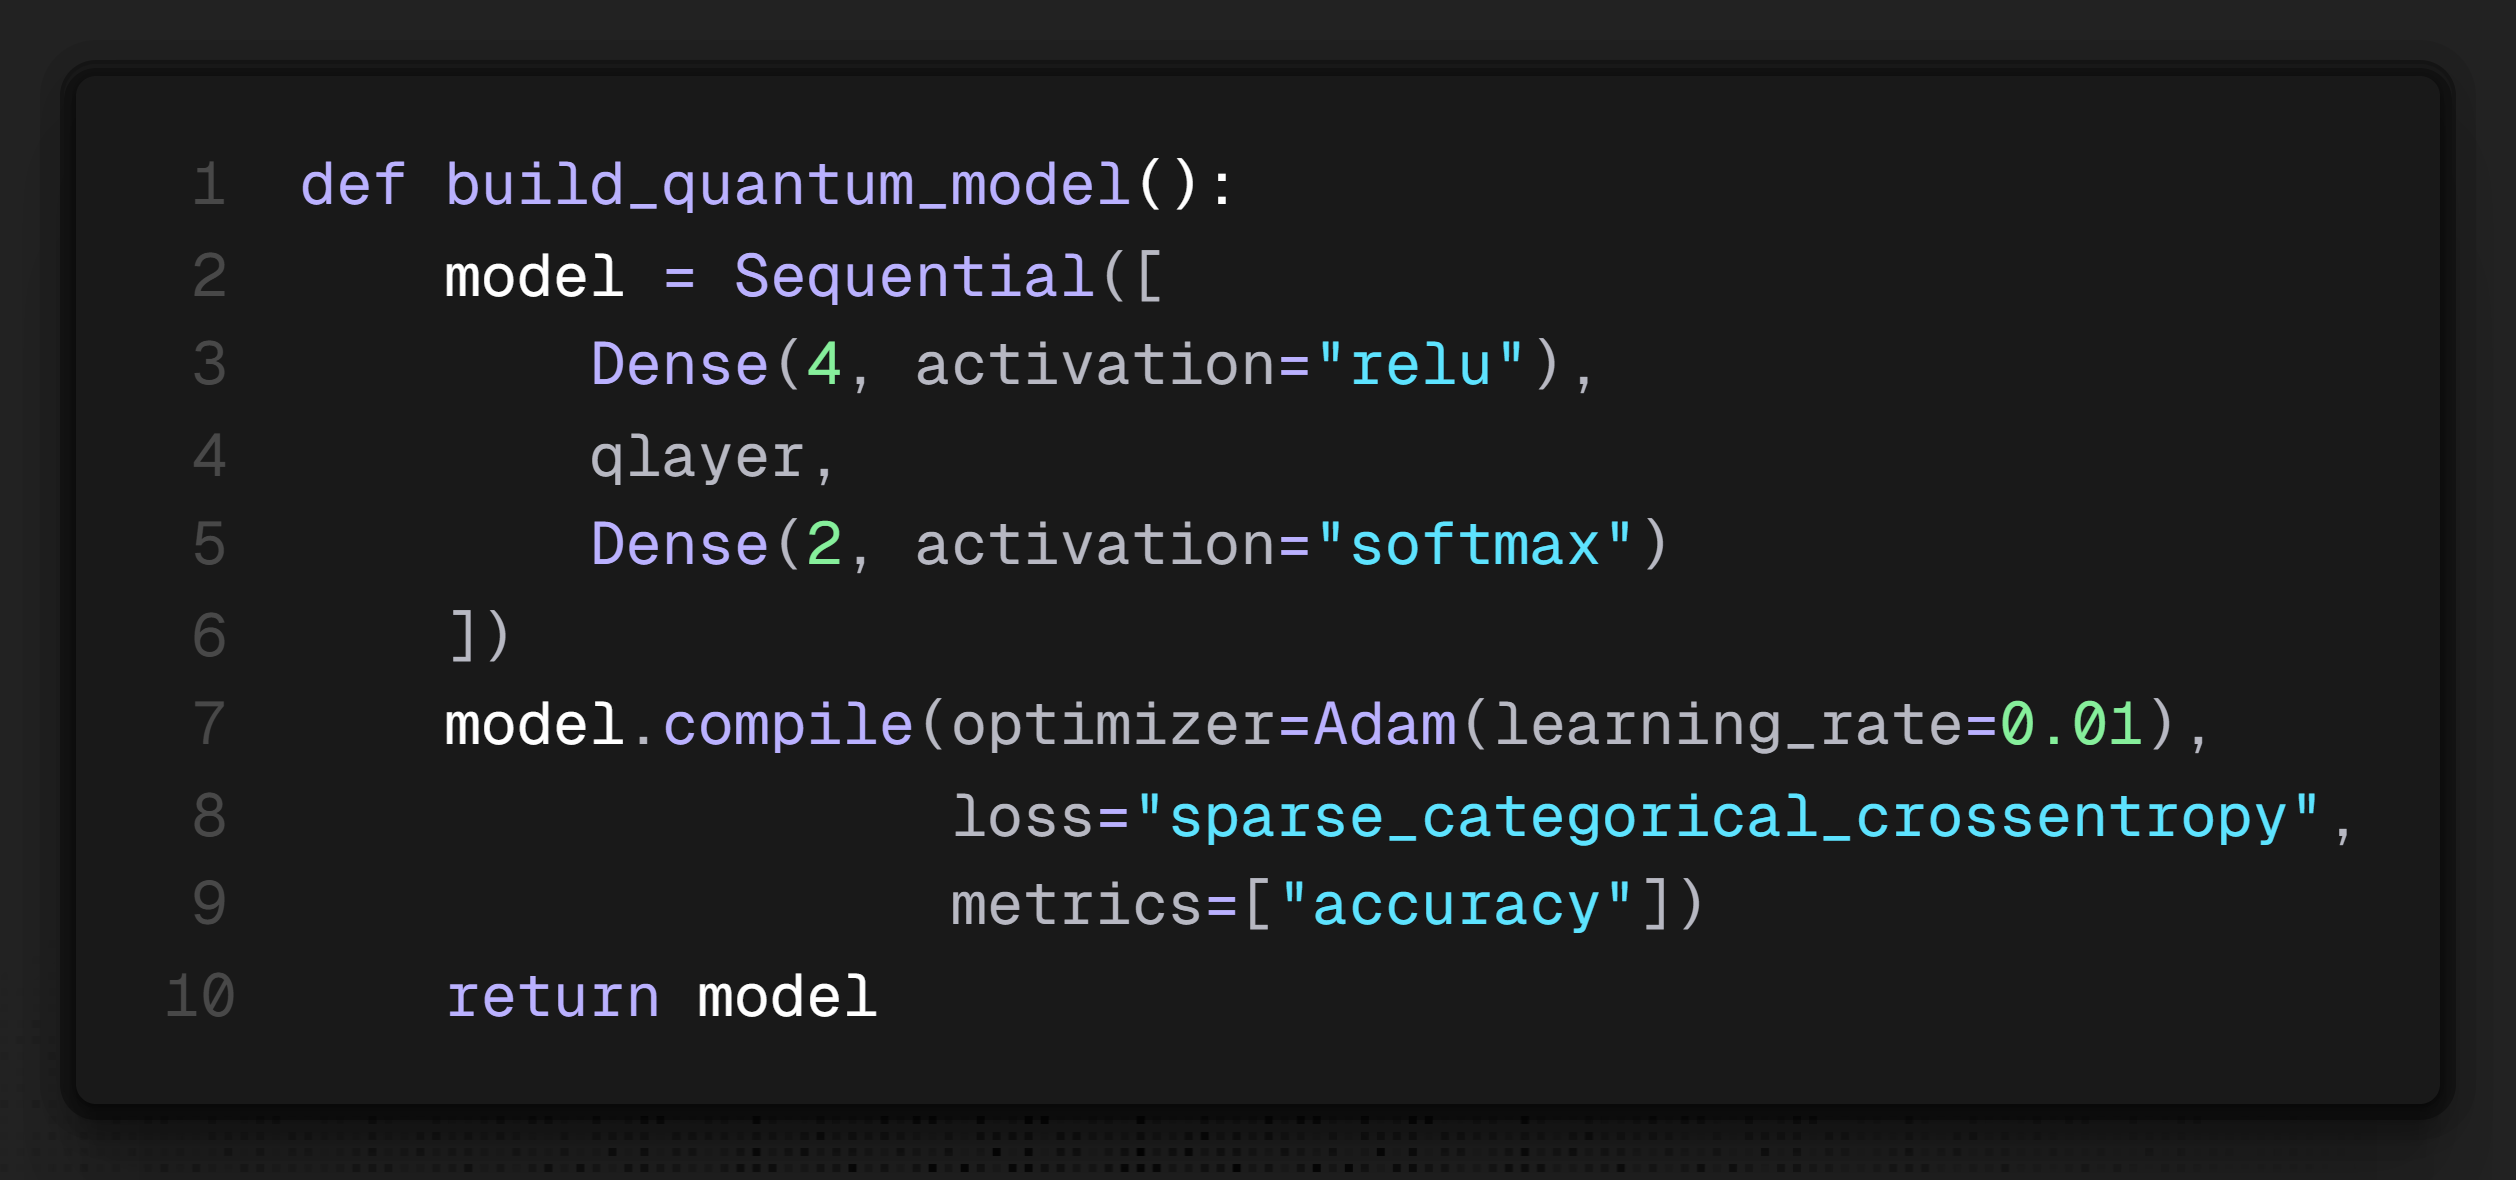
\includegraphics[height = 0.2\textheight]{img/QFL_code/6.png}
\end{figure}
The function \texttt{build\_quantum\_model()} constructs a hybrid neural network model that integrates classical dense layers with a trainable quantum layer.
The model architecture consists of three main components:
\begin{itemize}
	\item \texttt{Dense(4, activation="relu")} is the first classical layer with 4 neurons and ReLU activation. This layer performs a nonlinear transformation on the input data and projects it into a higher-dimensional space suitable for quantum processing.
	\item \texttt{qlayer} is a quantum layer instantiated using \texttt{qml.qnn.KerasLayer}, which wraps a quantum circuit defined via a QNode. This layer accepts classical input, encodes it into quantum states (e.g., via AngleEmbedding), applies the trainable quantum circuit (such as \texttt{custom\_layer\_long}), and returns classical output via expectation measurements.
	\item \texttt{Dense(2, activation="softmax")} is the final classical layer that maps the quantum output to a 2-dimensional vector suitable for binary classification. The \texttt{softmax} activation ensures that the outputs are normalized and interpretable as class probabilities.
\end{itemize}
The model is compiled using the Adam optimizer with a learning rate of 0.01, and it employs the categorical cross-entropy loss function.
In the next step, we will implement the local training process for each client.

\paragraph{Secure Weight Extraction and Encryption.}
After local training, the weights of each client's model are extracted specifically from the dense layers. These weights are first split using Shamir’s Secret Sharing scheme, which converts each real-valued weight into a set of $n$ modular shares using a polynomial of degree $k - 1$. This ensures that the weight can only be reconstructed if at least $k$ out of $n$ shares are collected. The integer conversion via multiplication by $10^6$ maintains precision while ensuring compatibility with modular arithmetic over a prime field.
Subsequently, the original weight matrices are also encrypted using the CKKS (Cheon–Kim–Kim–Song) homomorphic encryption scheme. This encryption allows computation directly on ciphertexts, meaning that model aggregation and analysis can be performed securely without decryption. The CKKS context is initialized with high-precision parameters suitable for approximate floating-point computation.
\begin{figure}[H]
	\centering
	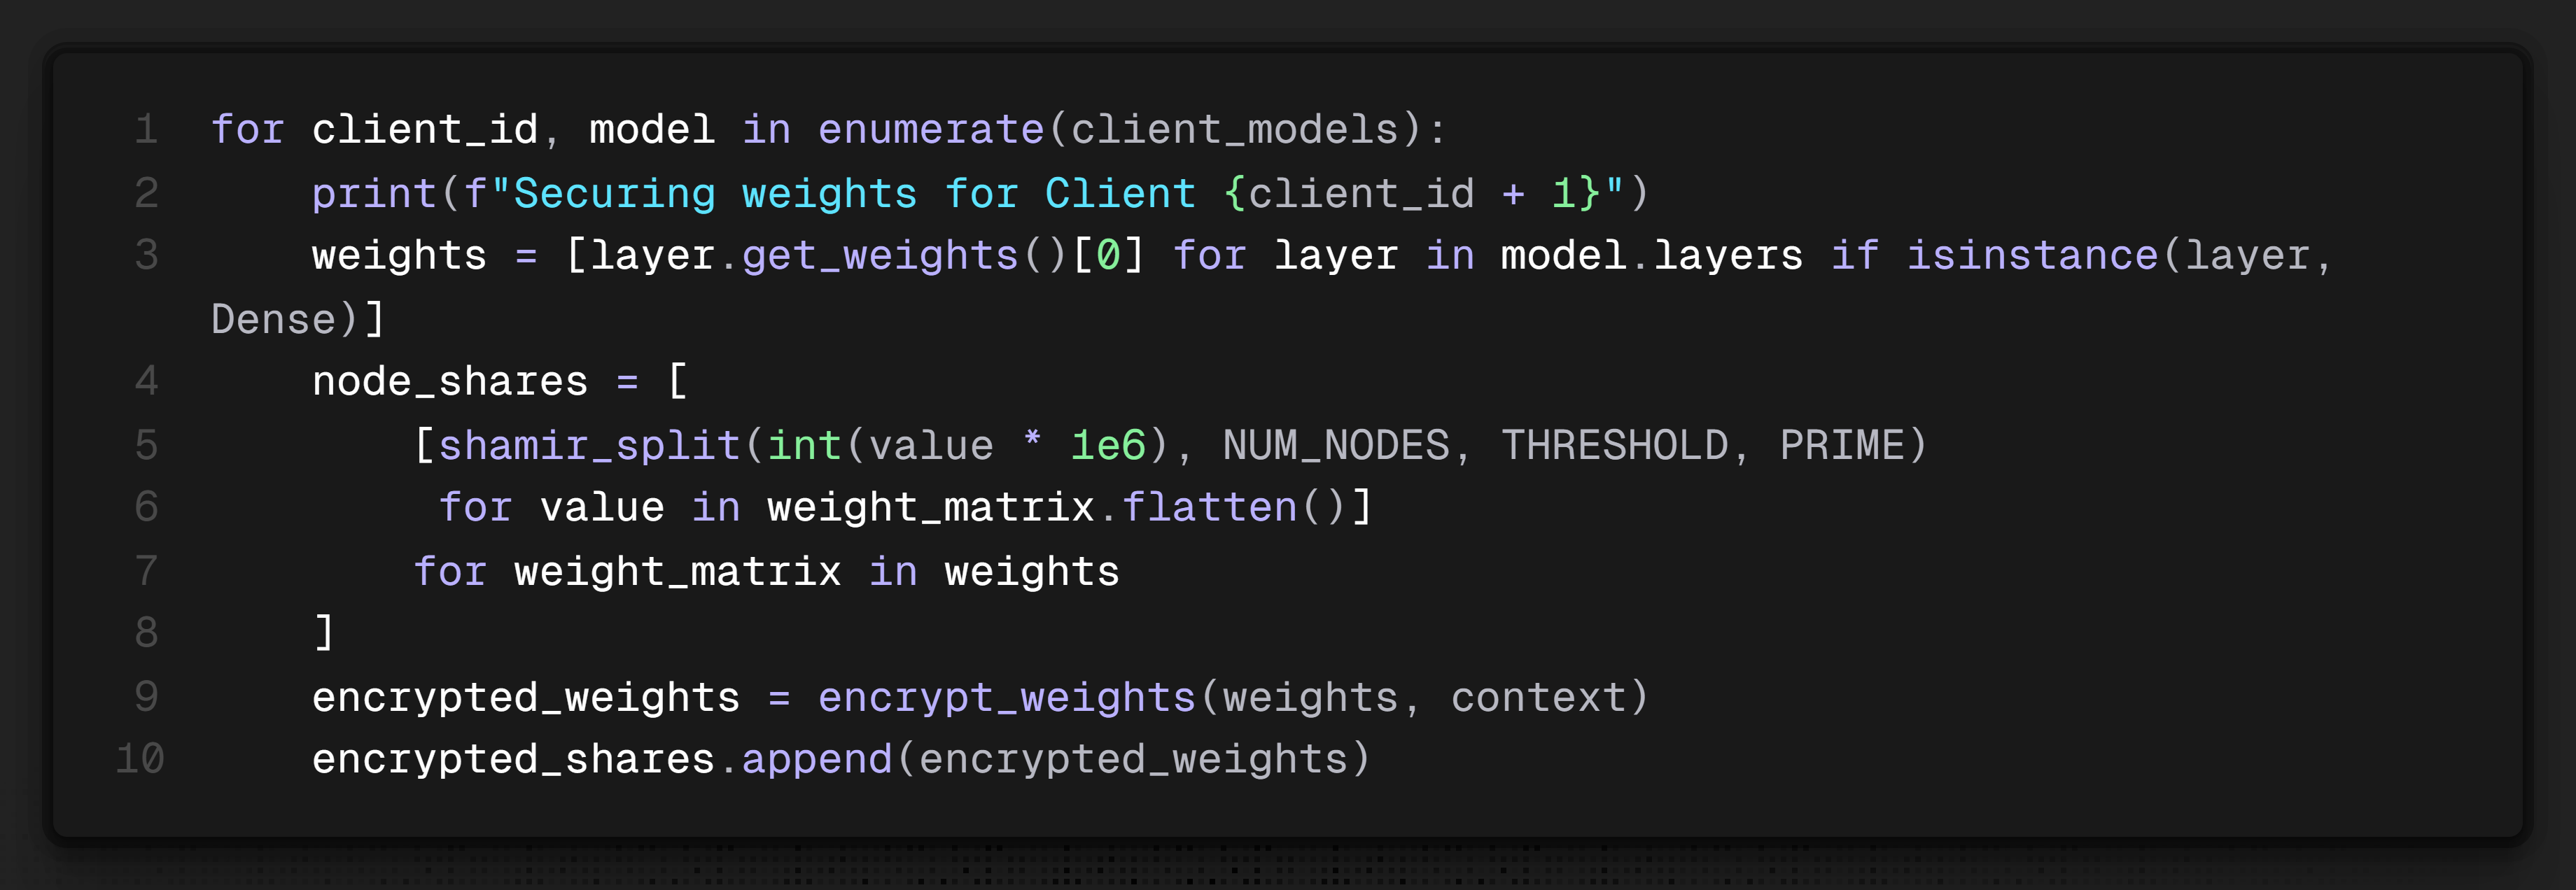
\includegraphics[height = 0.2\textheight]{img/QFL_code/7.png}
\end{figure}


\paragraph{Homomorphic Aggregation via Weighted Median.}
To construct a new global model from the encrypted local updates, a weighted median aggregation is performed directly in the encrypted domain. Each client's contribution is scaled using an adaptive factor, which reflects dynamic properties such as data quality, trust level, or sample size.\\
The encrypted weights are first decrypted temporarily (within the secure enclave of the aggregation server) to perform the median operation. For each position in the weight vector, values from all clients are collected, sorted, and the weighted cumulative distribution is computed. The value corresponding to the median weight threshold (typically at cumulative weight $\geq 0.5$) is then selected as the aggregate for that parameter. This robust aggregation reduces the influence of outliers or malicious updates while preserving differential weight importance.
\begin{figure}[H]
	\centering
	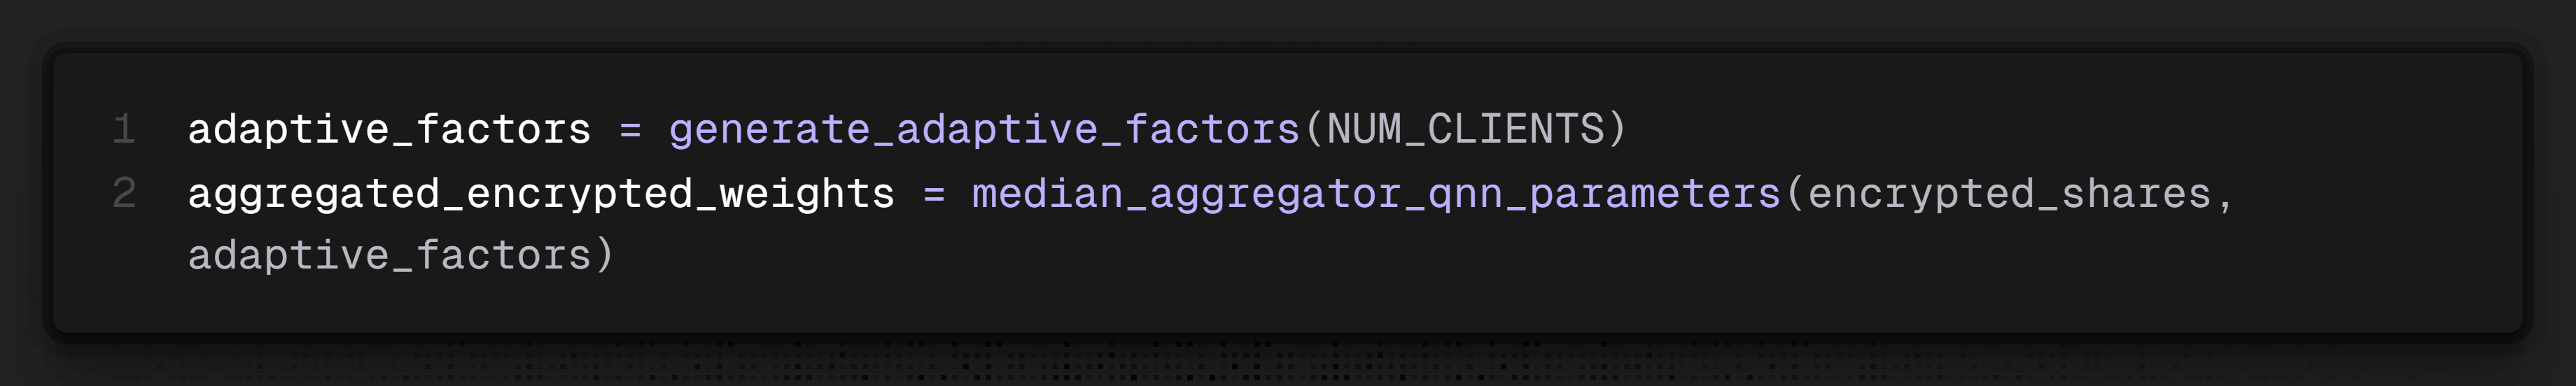
\includegraphics[height = 0.08\textheight]{img/QFL_code/9.png}
\end{figure}

\paragraph{Simulated QKD and AES-Based Model Distribution.}
To securely distribute the newly aggregated global model to all clients, a Quantum Key Distribution (QKD) simulation is employed. In this setup, each client is assigned a unique 128-bit AES key generated via a secure random process. Although not a true quantum system, this approach mimics the security properties of QKD by assuming an independent, pre-shared key per node.
The global model is serialized into 32-bit floats and encrypted block-wise using AES in ECB mode with PKCS7 padding. This encryption guarantees that only the intended client, with access to its unique key, can decrypt and load the model update.
\begin{figure}[H]
	\centering
	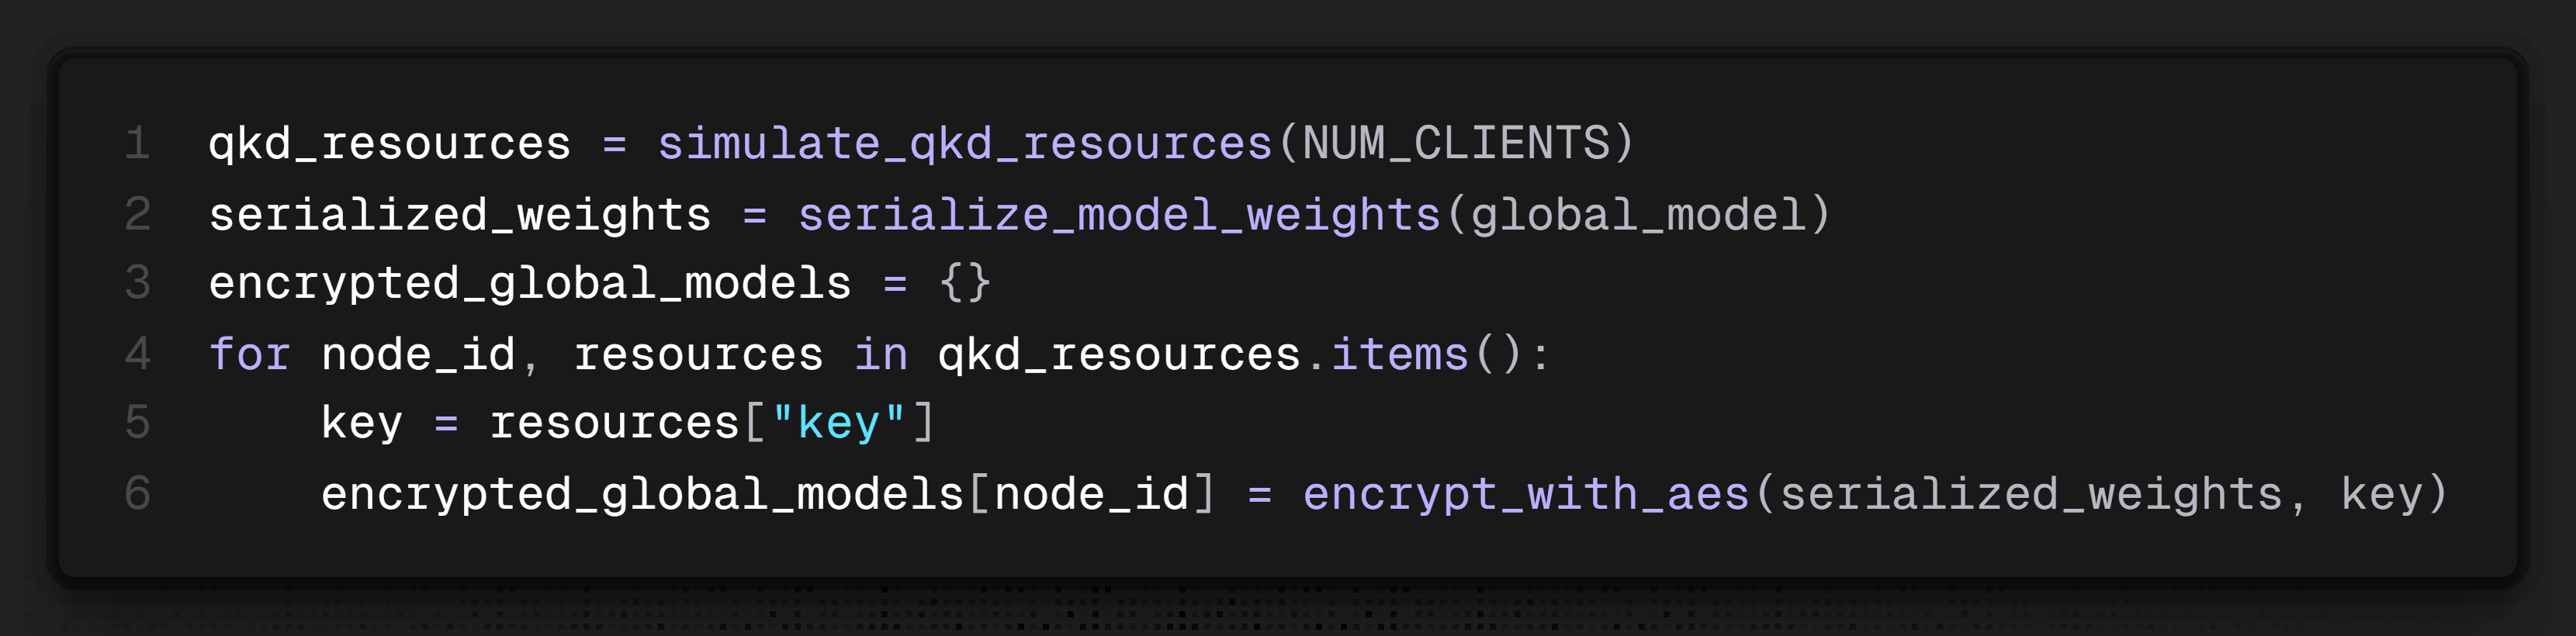
\includegraphics[height = 0.15\textheight]{img/QFL_code/10.png}
\end{figure}

\paragraph{Evaluation of Aggregated and Local Models.}
After each training and aggregation round, the global model is evaluated on a test set consisting of all clients’ data. This provides a comprehensive metric of generalization across the entire system. Simultaneously, the performance of an individual client (typically Client 1) is also assessed on its own local test set to monitor personalized model performance.
The results from each iteration are stored for both global and local accuracy, enabling longitudinal analysis of the model's evolution, convergence behavior, and fairness across clients.
\subsection{Results}
\begin{figure}[H]
	\centering
	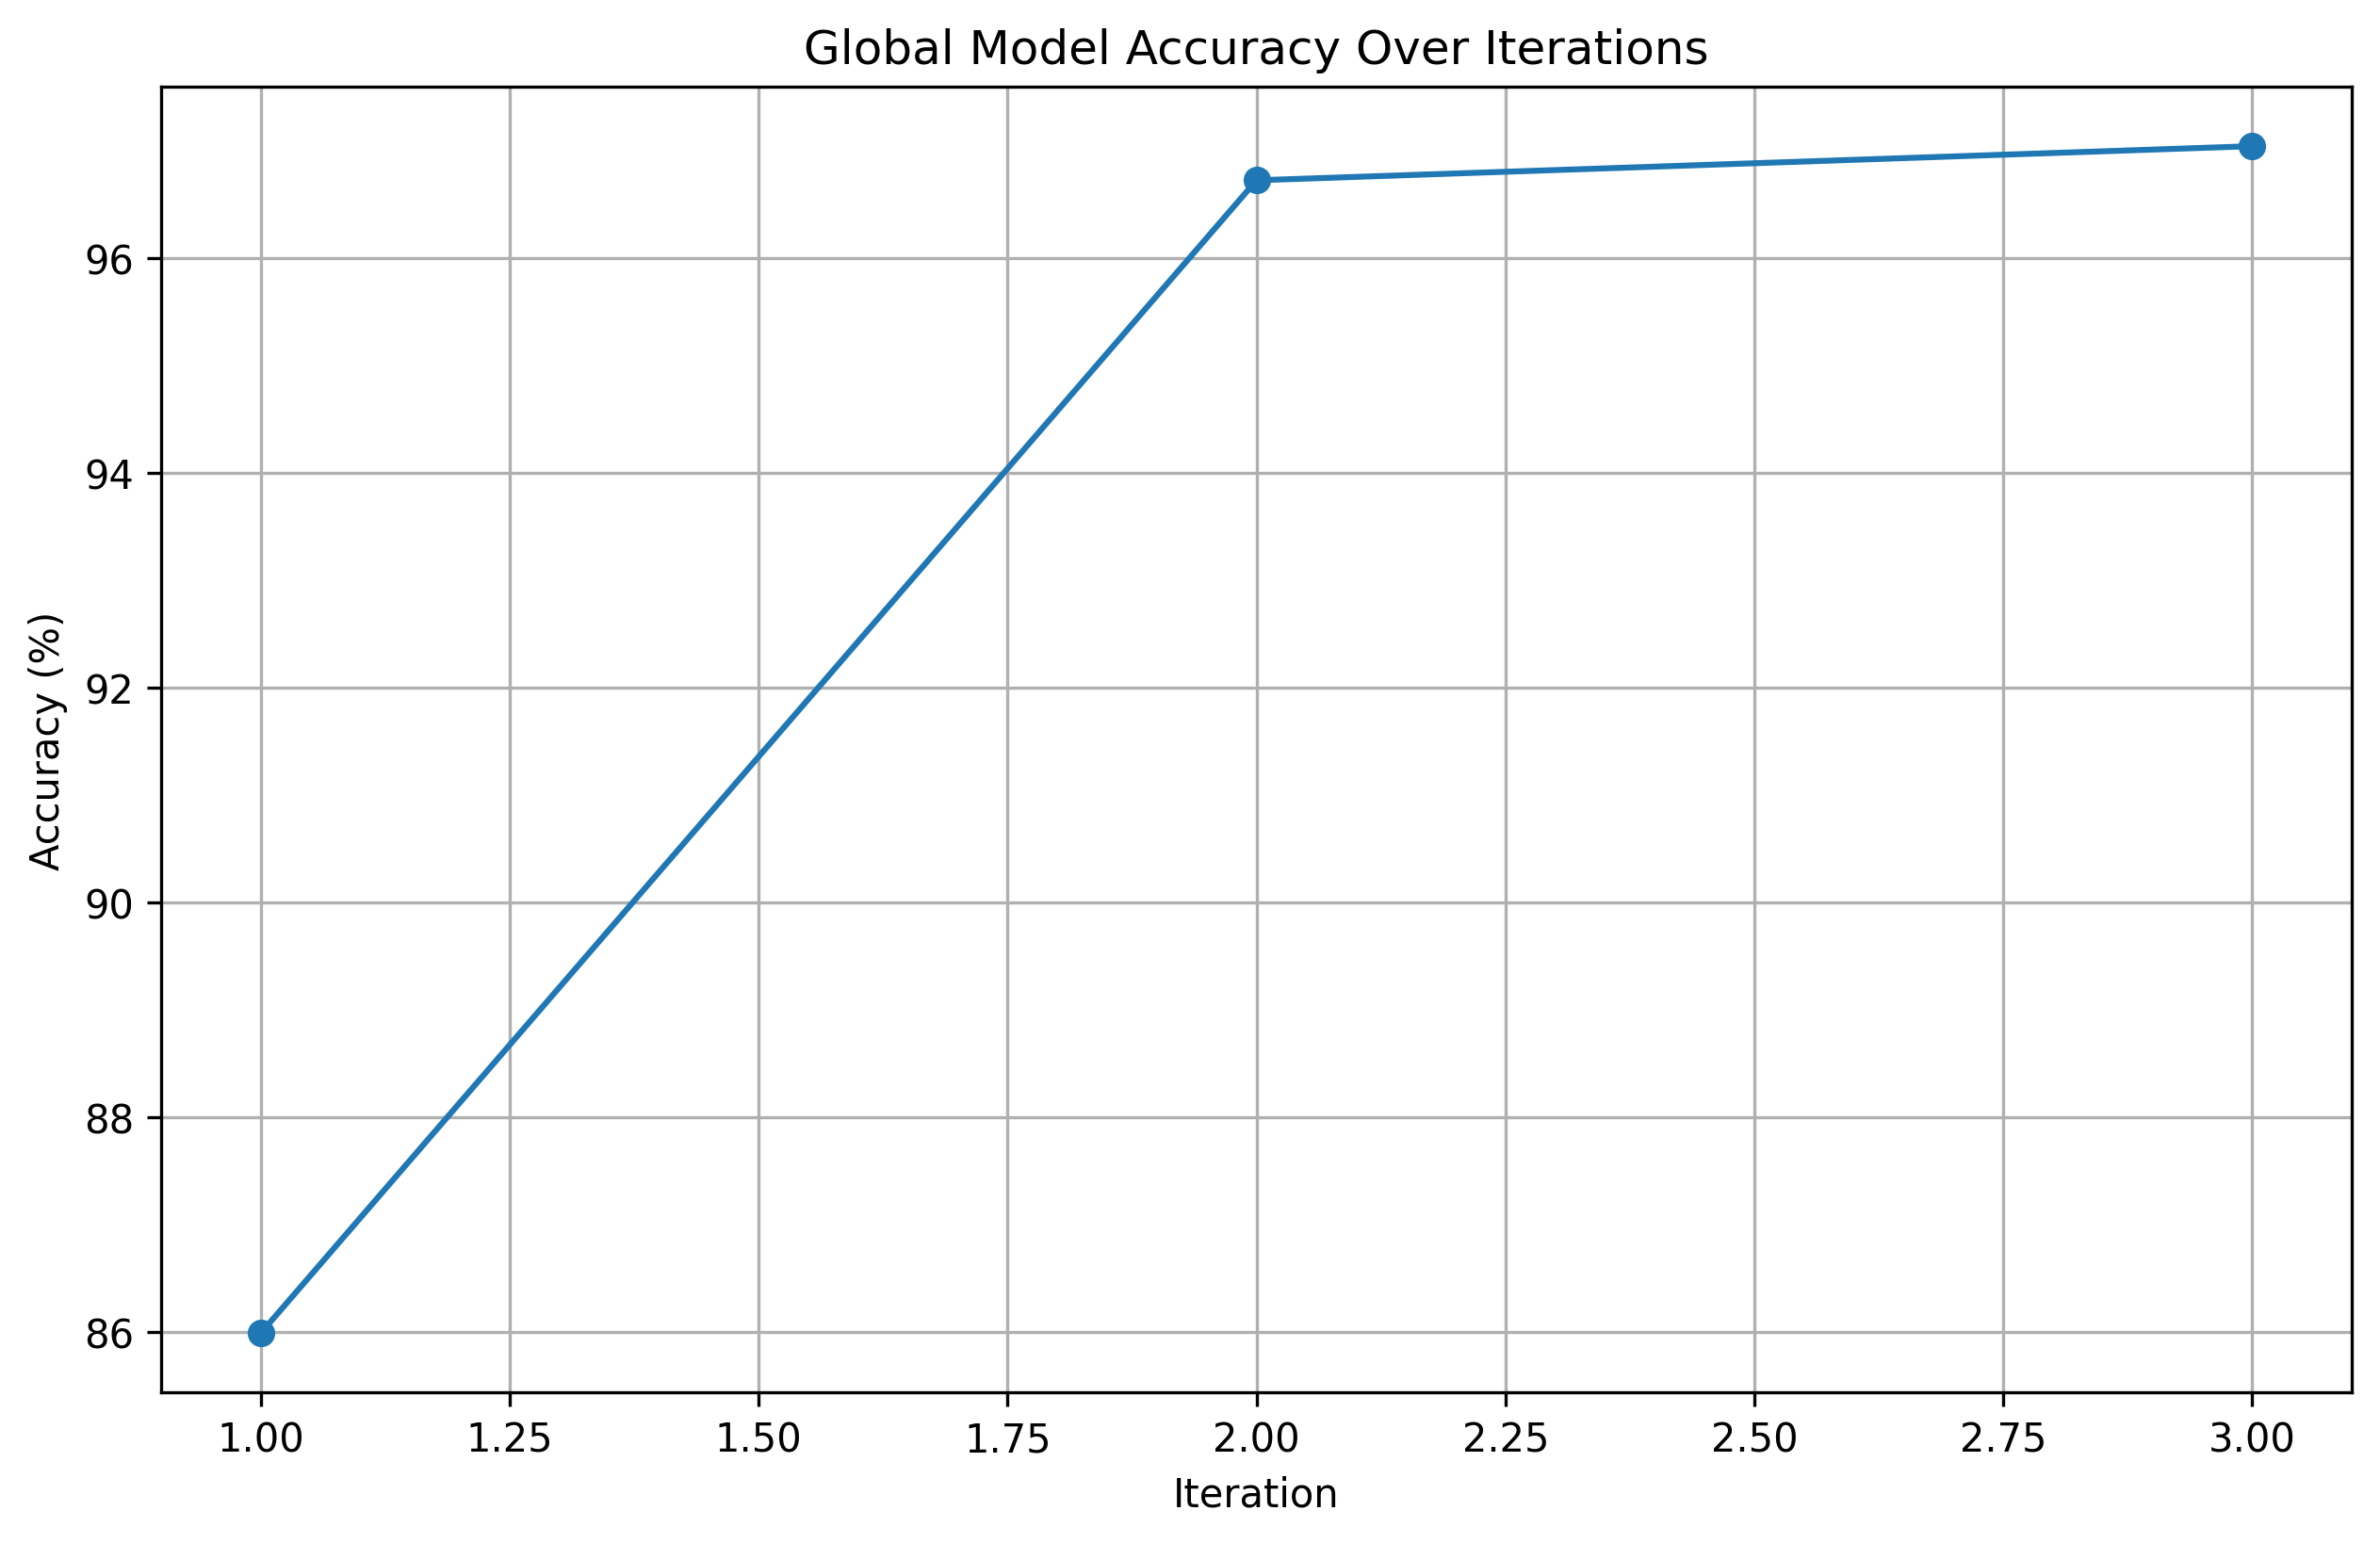
\includegraphics[height = 0.4\textheight]{img/global_model_accuracy.png}
    \caption{Global model accuracy on combined test set = 98.83\%}
\end{figure}
\begin{figure}[H]
    \centering
    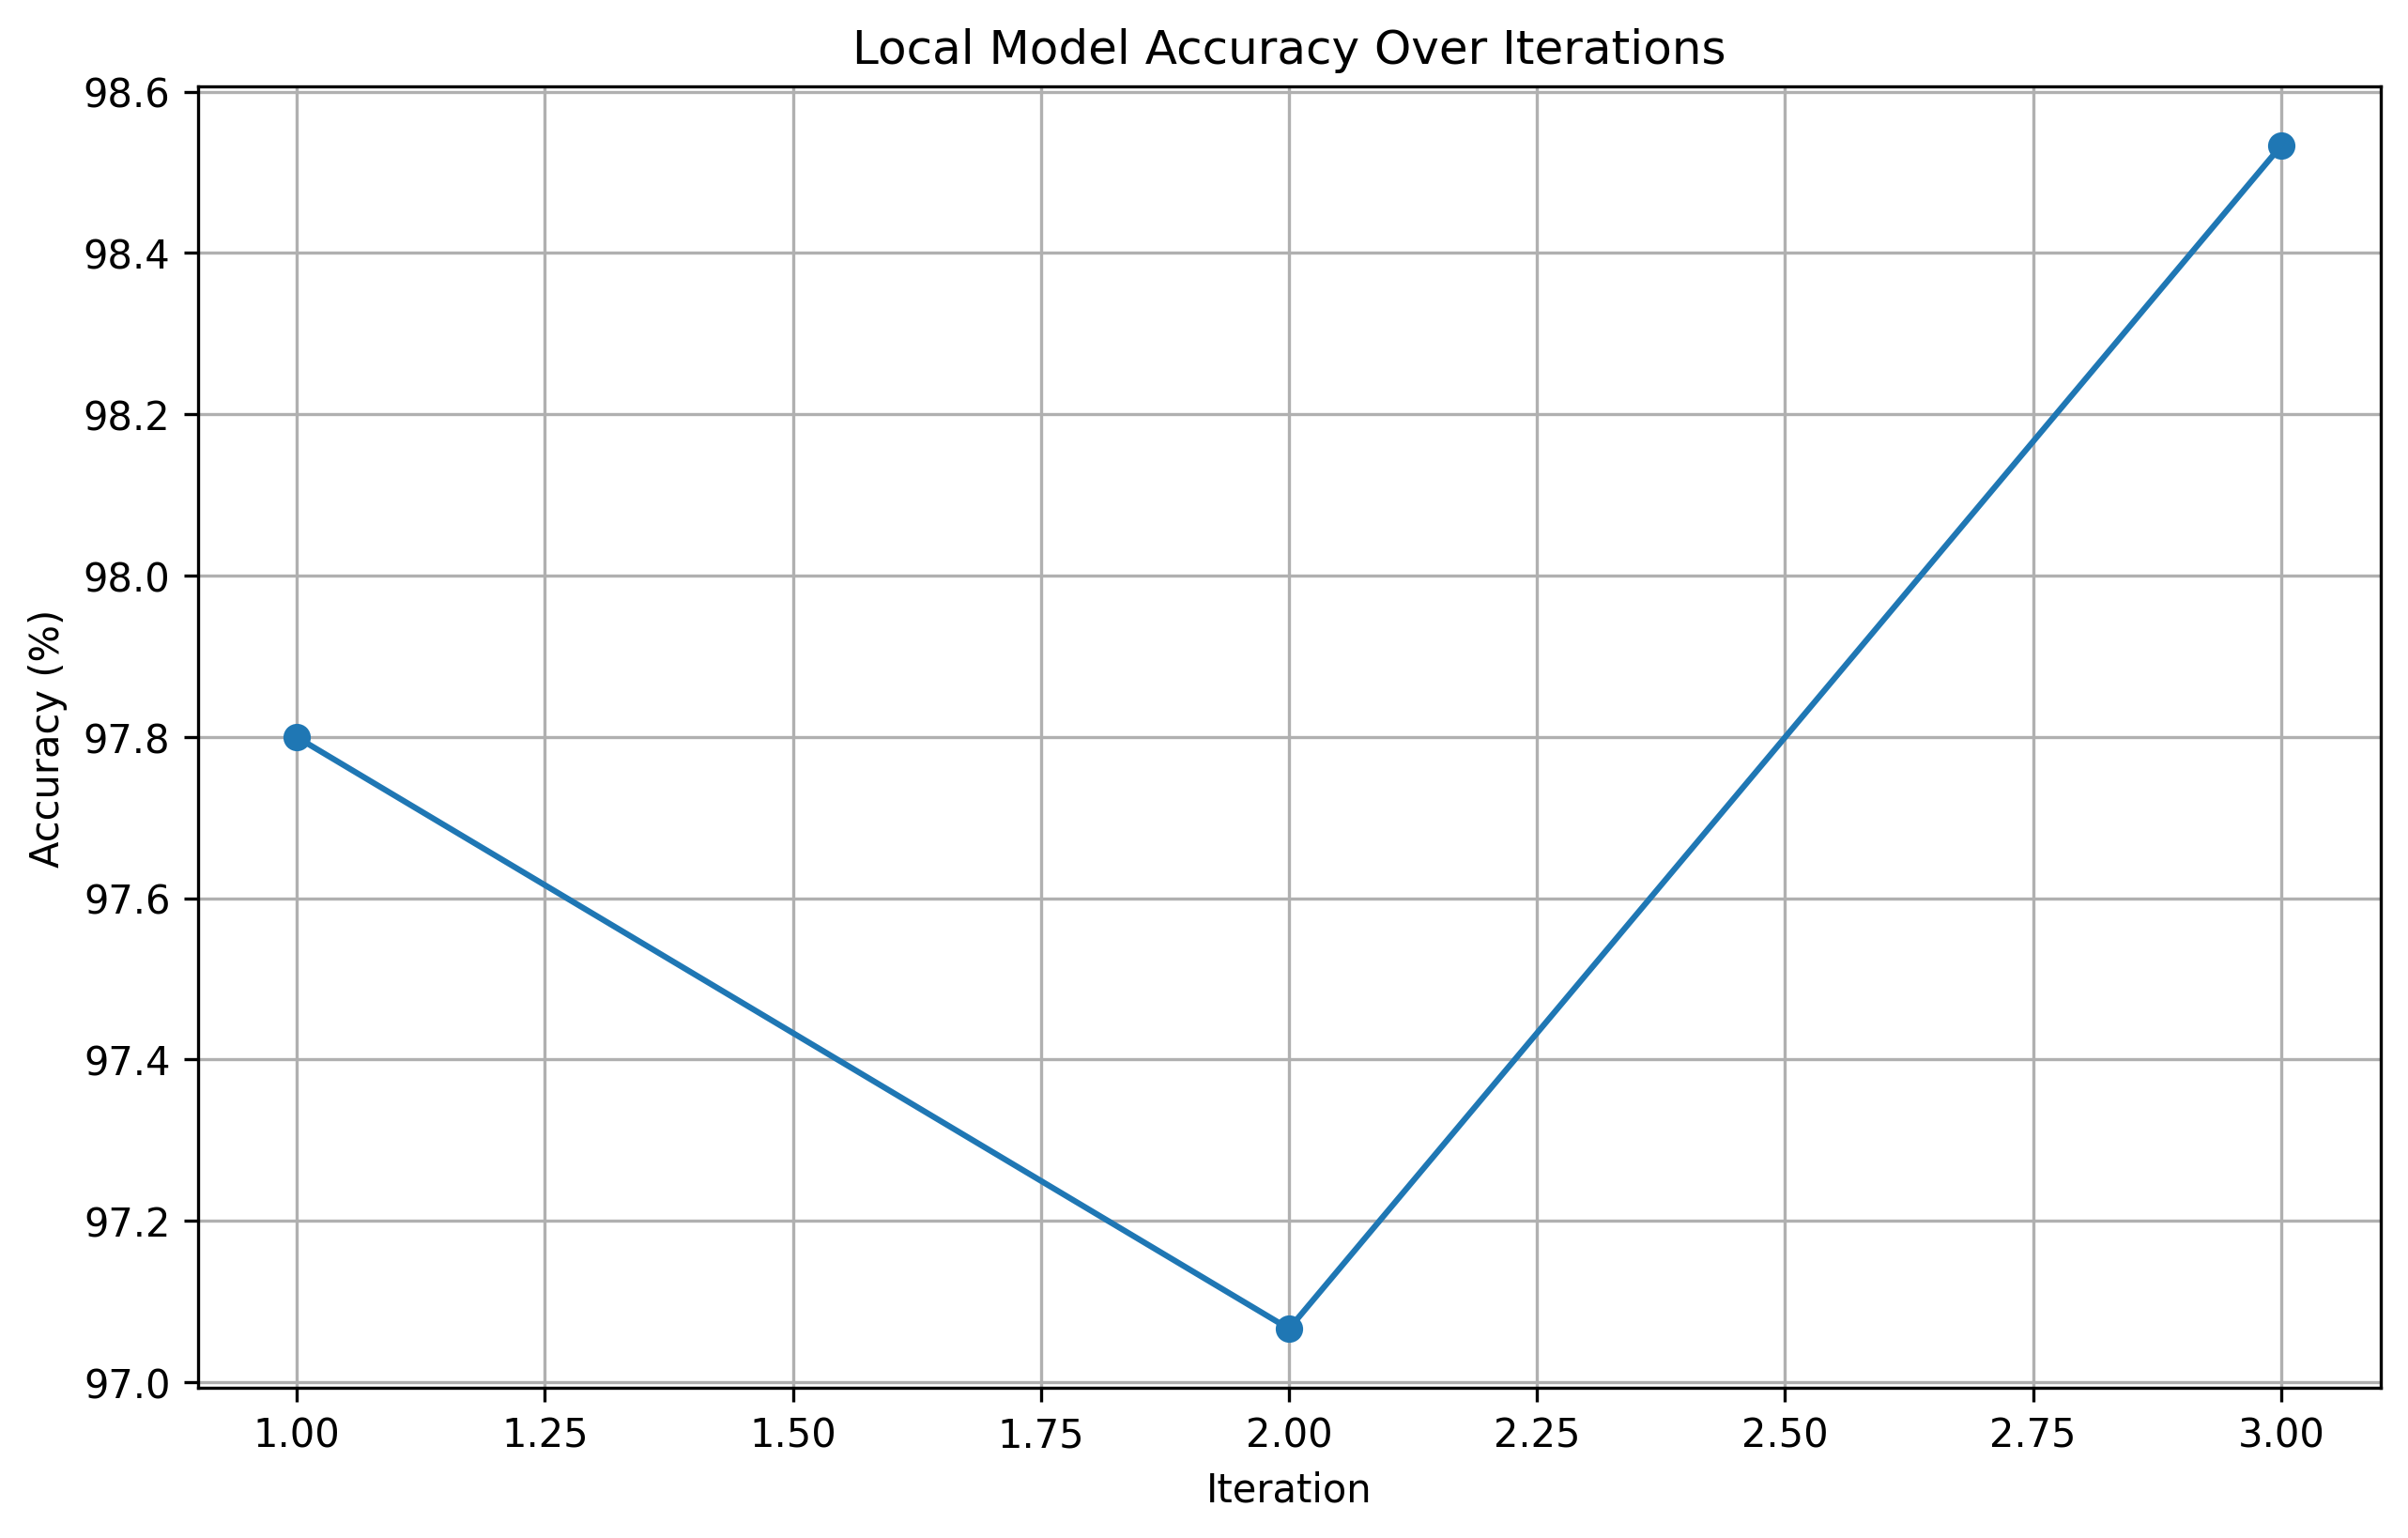
\includegraphics[height = 0.4\textheight]{img/local_model_accuracy.png}
    \caption{Client 1 model accuracy on its own test set = 98.53\%}
\end{figure}


\section{Conclusion}


\bibliographystyle{plain}
\bibliography{qml_project}

\end{document}
